\documentclass{beamer}
\usepackage{ctex, hyperref}
\usepackage[T1]{fontenc}

% other packages
\usepackage{latexsym,amsmath,xcolor,multicol,booktabs,calligra}
\usepackage{graphicx,pstricks,listings,stackengine}

\author{Huchi}
\title{Retrieval-Based Chatbot}
\subtitle{Task Introduction and Next Work}
\institute{Natural Language Processing Research Group \\  Nanjing University}
\date{11/5/2020}
\usepackage{nju}

% defs
\def\cmd#1{\texttt{\color{red}\footnotesize $\backslash$#1}}
\def\env#1{\texttt{\color{blue}\footnotesize #1}}
\definecolor{deepblue}{rgb}{0,0,0.5}
\definecolor{deepred}{rgb}{0.6,0,0}
\definecolor{deepgreen}{rgb}{0,0.5,0}
\definecolor{halfgray}{gray}{0.55}

\lstset{
    basicstyle=\ttfamily\small,
    keywordstyle=\bfseries\color{deepblue},
    emphstyle=\ttfamily\color{deepred},    % Custom highlighting style
    stringstyle=\color{deepgreen},
    numbers=left,
    numberstyle=\small\color{halfgray},
    rulesepcolor=\color{red!20!green!20!blue!20},
    frame=shadowbox,
}


\begin{document}

\kaishu
\begin{frame}
    \titlepage
    \begin{figure}[htpb]
        \begin{center}
            % \includegraphics[width=0.2\linewidth]{pic/Tsinghua_University_Logo.eps}
        \end{center}
    \end{figure}
\end{frame}

\begin{frame}
    \tableofcontents[sectionstyle=show,subsectionstyle=show/shaded/hide,subsubsectionstyle=show/shaded/hide]
\end{frame}


\section{Task Introduction}

% \begin{frame} {Multi-turn Response Selection问题定义}
% 假设有数据集 $\mathcal{D}=\left\{\left(y_{i}, s_{i}, r_{i}\right)\right\}_{i=1}^{N},$ 其中 $s_{i}$ 对话上下文文本信息, $r_{i}$ 是一个回复的候选项,  $y_{i} \in\{0,1\}$ 是标签. $s_{i}=\left\{u_{i, 1}, \ldots, u_{i, n_{i}}\right\}$ 其中 $\left\{u_{i, k}\right\}_{k=1}^{n_{i}}$ 是每一轮的语句。
% \\
% $\forall k, u_{i, k}=\left(w_{u_{i, k}, 1}, \ldots, w_{u_{i, k}, j}, \ldots, w_{u_{i, k}, n_{u_{i}, k}}\right)$ 其中 $w_{u_{i, k}, j}$ 是第 $j$ 个词在 $u_{i, k}$ 中且, $n_{u_{i}, k}$ 是 $u_{i, k} $的长度. 同样的, $r_{i}=\left(w_{r_{i}, 1}, \ldots, w_{r_{i}, j}, \ldots, w_{r_{i}, n_{r_{i}}}\right)$ 其中 $w_{r_{i}, j}$ 是第 $j$ 个词在 $r_{i}$ 中且 $n_{r_{i}}$ 是回复语句的长度. $y_{i}=1$ 则说明 $r_{i}$ 是一个正确的回复对于 $s_{i}$, 否则 $y_{i}=0 $。 
% \\
% 我们的目标是学习一个匹配模型 $g(\cdot, \cdot)$ 在数据集 $\mathcal{D}$ 上, 并且对于任何新的匹配对 $(s, r)$, 可以测量他们的匹配程度$g(s, r)$. 根据 $g(s, r),$ 我们可以根据 $s$ 的候选项进行排序 并且选择一个正确的作为回复。
% \end{frame}

\subsection{Problem Formalization}
\begin{frame} {Multi-turn Response Selection Problem Formalization}
Suppose that we have a data set $\mathcal{D}=\left\{\left(y_{i}, s_{i}, r_{i}\right)\right\}_{i=1}^{N},$ where $s_{i}$ is a conversation context, $r_{i}$ is a response candidate, and $y_{i} \in\{0,1\}$ is a label. $s_{i}=\left\{u_{i, 1}, \ldots, u_{i, n_{i}}\right\}$ where $\left\{u_{i, k}\right\}_{k=1}^{n_{i}}$ are utterances. $y_{i}=1$ if $r_{i}$ is a proper response to $s_{i}$, otherwise $y_{i}=0 .$ 
\\
Our goal is to \textbf{learn a matching model $g(\cdot, \cdot)$} with $\mathcal{D},$ and thus for any new context-response pair $(s, r), g(s, r)$ measures their matching degree. According to $g(s, r),$ we can rank candidates for $s$ and select a proper one as its response.
\end{frame}

\subsection{Dataset Introduction}
\begin{frame}{Dataset Brief Introduction}
    \begin{itemize}
        \item English
        \begin{itemize}
            \item 2015 Ubuntu Dialogue Corpus v1.0 Dialogs: 930K
            \item 2018 DSTC7-Ubuntu 5 subtasks
            \item 2018 Persona-Chat  Dialogs: Train/Valid/Test: 10907/1000/968, Personas: 1155
            \item 2015-2019 PolyAI-Reddit Train/Test: 654M/72M
        \end{itemize}
        \item Chinese
        \begin{itemize} 
            \item 2016 Douban Train/Valid/Test: 1M/50K/10K
            \item 2020 LCCC Base/Large: 6M/12M
        \end{itemize}
        
    \end{itemize}
\end{frame}


\section{Research Status}

\subsection{Framework for the Existing Models}


\begin{frame}{A Framework for the Existing Models: Bi-Encoder}
     \begin{center}
    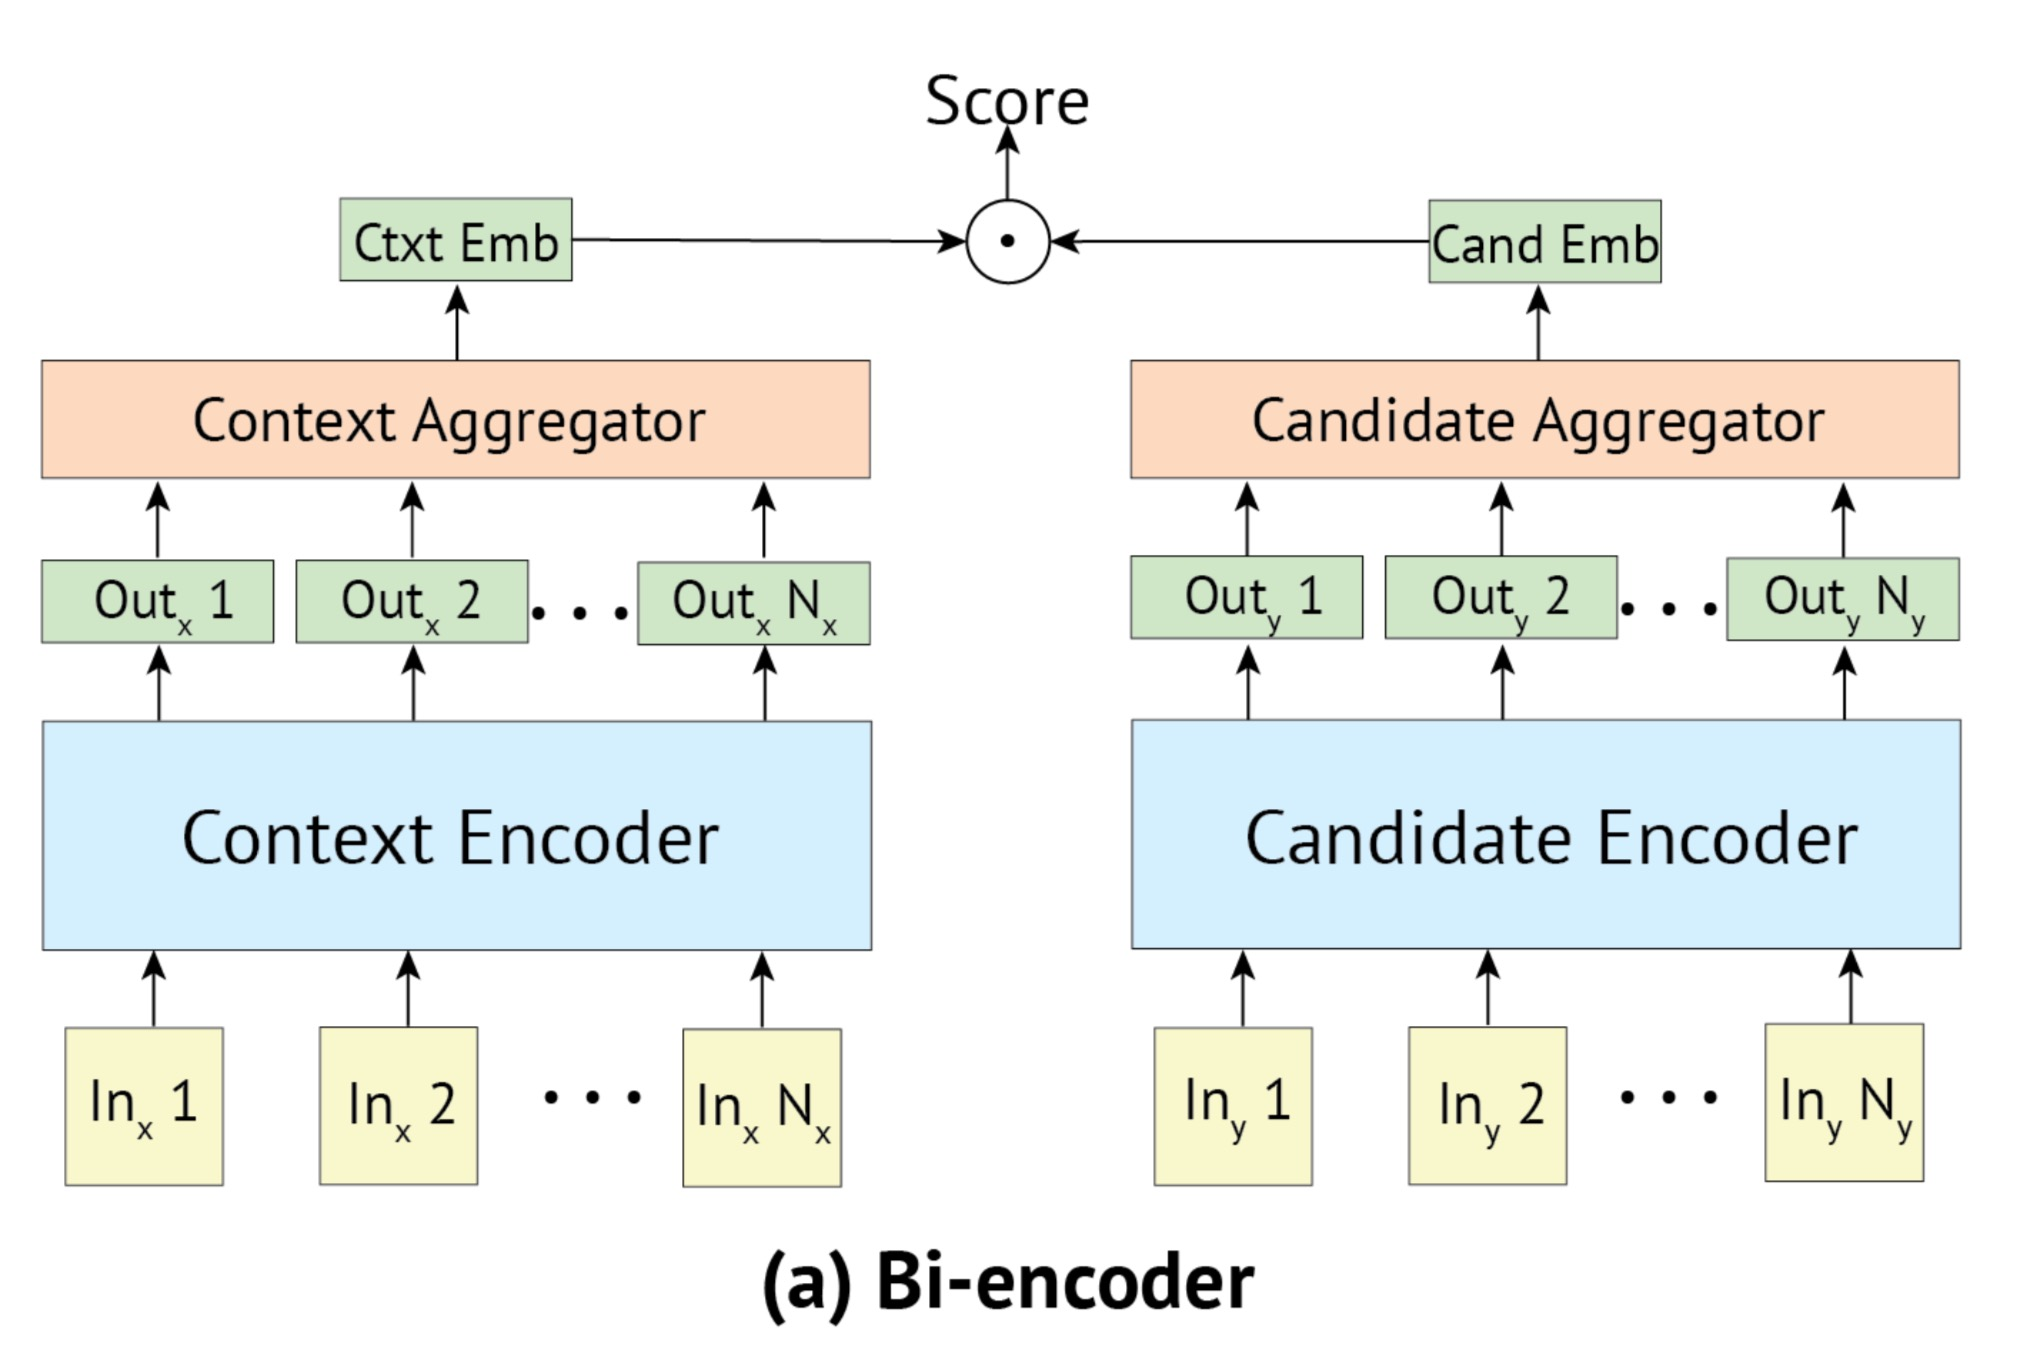
\includegraphics[width=0.9\linewidth]{Bi-encoder.png}
     \end{center}
\end{frame}

\begin{frame}{A Framework for the Existing Models: Cross-Encoder}
     \begin{center}
    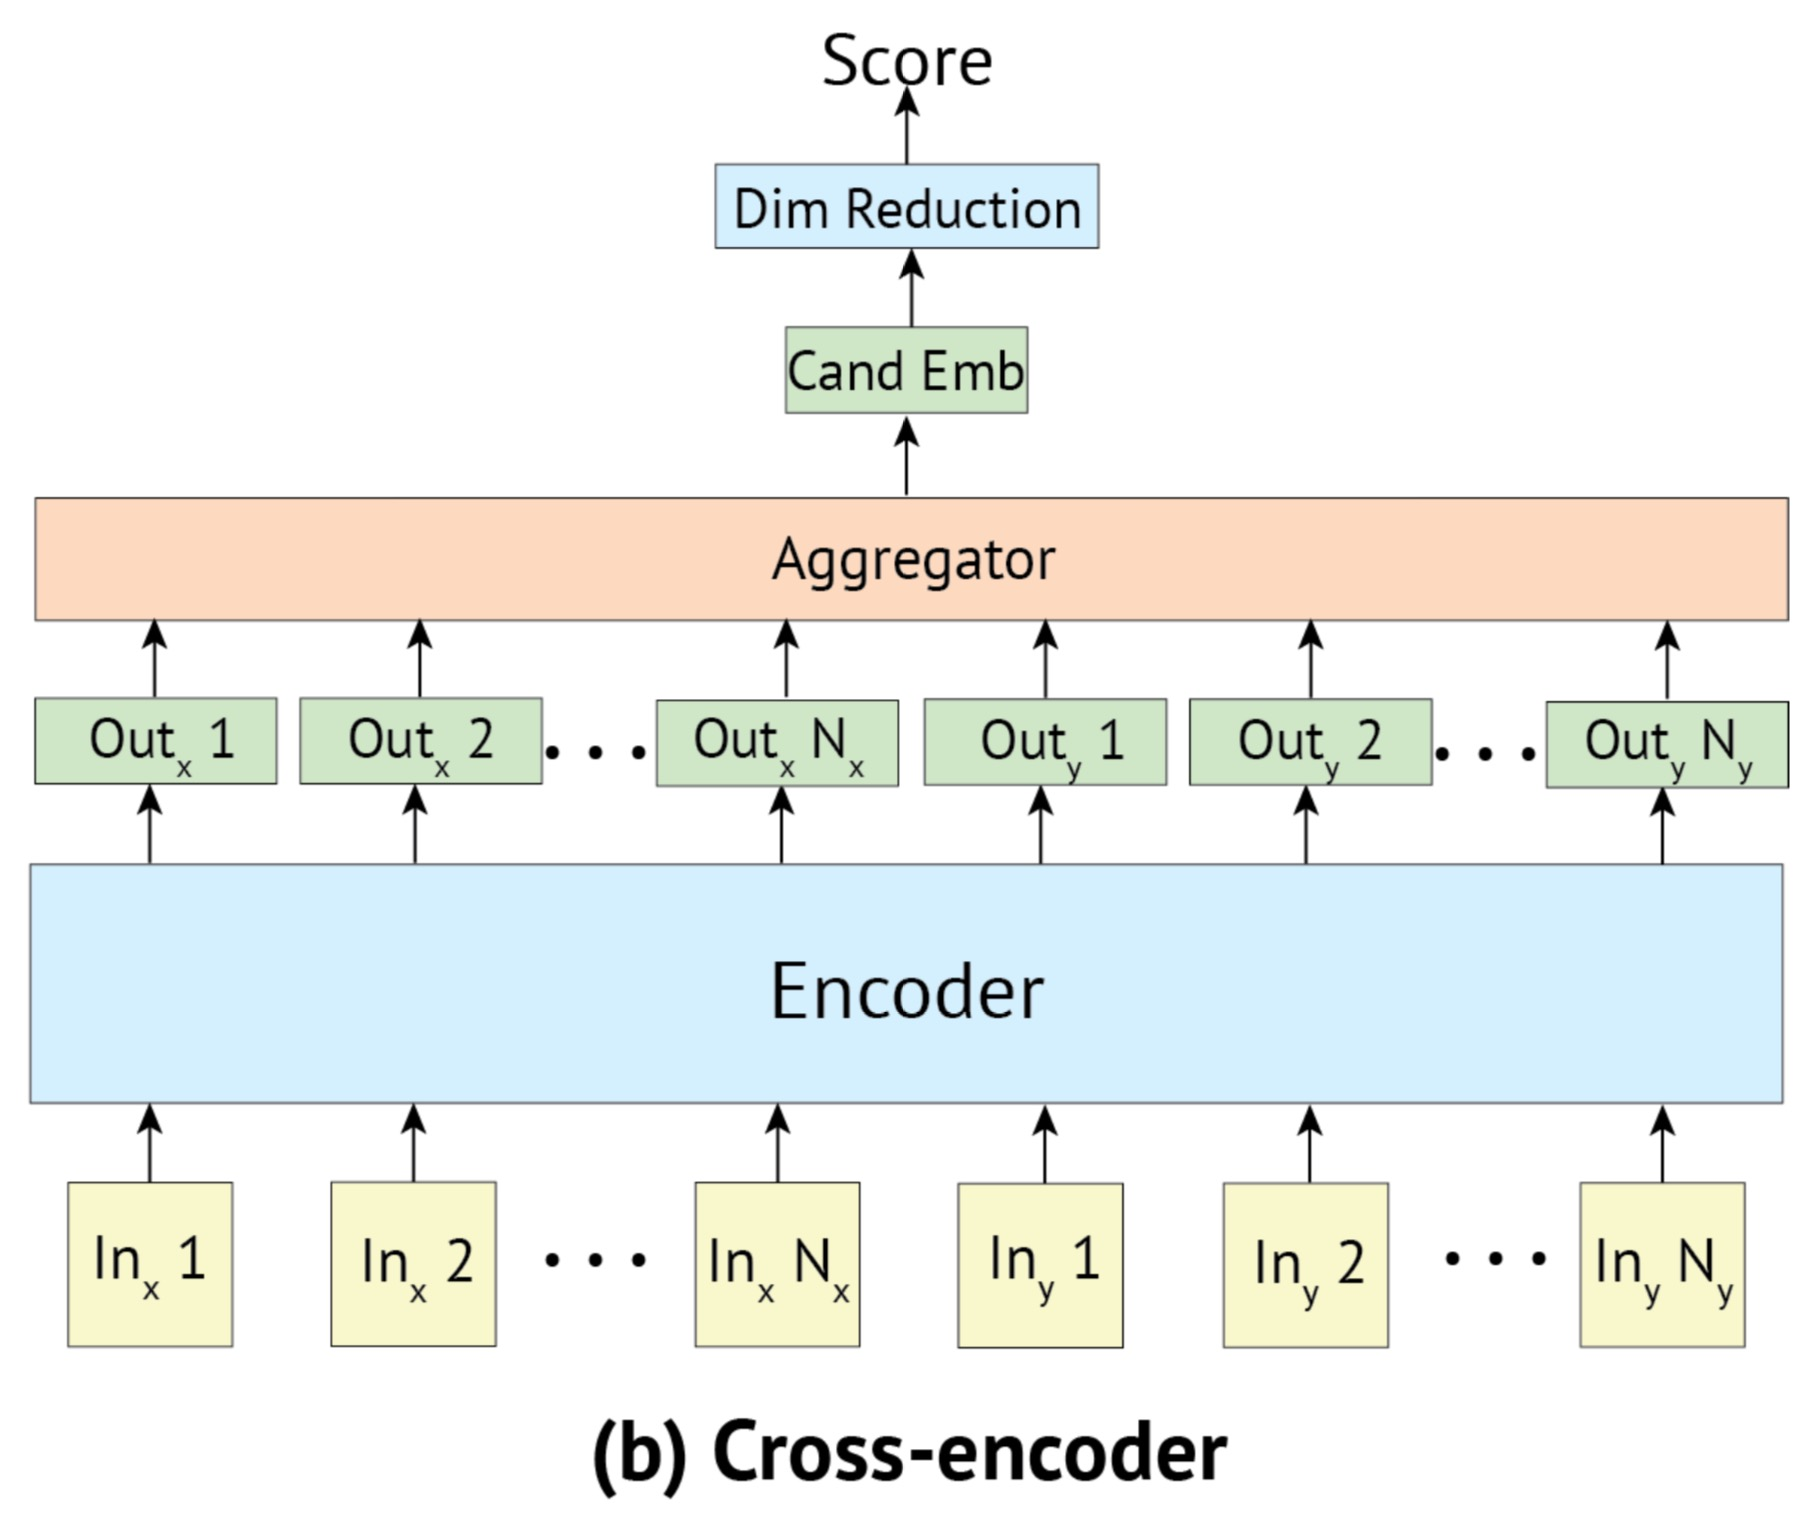
\includegraphics[width=0.75\linewidth]{Cross-encoder.png}
     \end{center}
\end{frame}

\begin{frame}{Difference between Bi-Encoder and Cross-Encoder}
    \begin{itemize}
        \item Since the candidate encodings are independent of the input, Bi-encoders are very \textbf{efficient during evaluation}. (cache the representations of a large, fixed candidate set)
        
        \item  Urbanek et al. (2019) finds that Cross-encoders \textbf{perform better} while the performance gains come at a steep computational cost. 
        
        \begin{tabular}{|c|c|c|c|c|}
\hline & \multicolumn{4}{|c|} { Scoring time (ms) } \\
\hline & \multicolumn{2}{|c|} { CPU } & \multicolumn{2}{c|} { GPU } \\
\hline Candidates & $1 \mathrm{k}$ & $100 \mathrm{k}$ & $1 \mathrm{k}$ & $100 \mathrm{k}$ \\
\hline \hline Bi-encoder & 115 & 160 & 19 & 22 \\
\hline Poly-encoder 360 & 160 & 837 & 57 & 88 \\
\hline Cross-encoder & $21.7 \mathrm{k}$ & $2.2 \mathrm{M}^{*}$ & $2.6 \mathrm{k}$ & $266 \mathrm{k}^{*}$ \\
\hline
\end{tabular}
        
    \end{itemize}
\end{frame}

\subsection{Recent Work Brief Introduction}
\begin{frame}{Recent Work Brief Introduction}
    \begin{itemize}
        \item ICLR 2020 Poly-Encoder 
            \begin{itemize}
                \item Pre-trained on 174 million examples extracted from Reddit with new strategies
                \item Propose Poly-Encoder which aims to get the best of both worlds from the Bi- and Cross-encoder
            \end{itemize}
        \item arXiv 2019 ConveRT
        \begin{itemize}
            \item Pre-trained on Reddit(727 million)
            \item Propose a compact dual-encoder pretraining architecture, leveraging subword representations, transformer-style blocks, and quantization
        \end{itemize}
        \item arXiv 2020 Bert-SL
        \begin{itemize}
            \item Propose \textbf{four self-supervised auxiliary tasks}, jointly train the PLM-based response selection model.
        \end{itemize}
    \end{itemize}
\end{frame}

\section{Difficulty In My Work}



% \begin{frame}{Difficult In My Work}
%     Dataset:
%     \begin{itemize}
%         \item 华为的微博数据 4M context-response pairs
%         \item 北航和微软的豆瓣多轮对话 1M context-response pairs
%         \item 清华的LCCC数据集 6.8M dialogs(Base), 12M dialogs(Large)
%     \end{itemize}
%     Problems:
%     \begin{itemize}
%         \item How to construct candidates whitelist?
%         \item 
%     \end{itemize}
% \end{frame}
\subsection{Core Problems}
\begin{frame}{Initially Immature Architecture}[htb]
     \begin{center}
        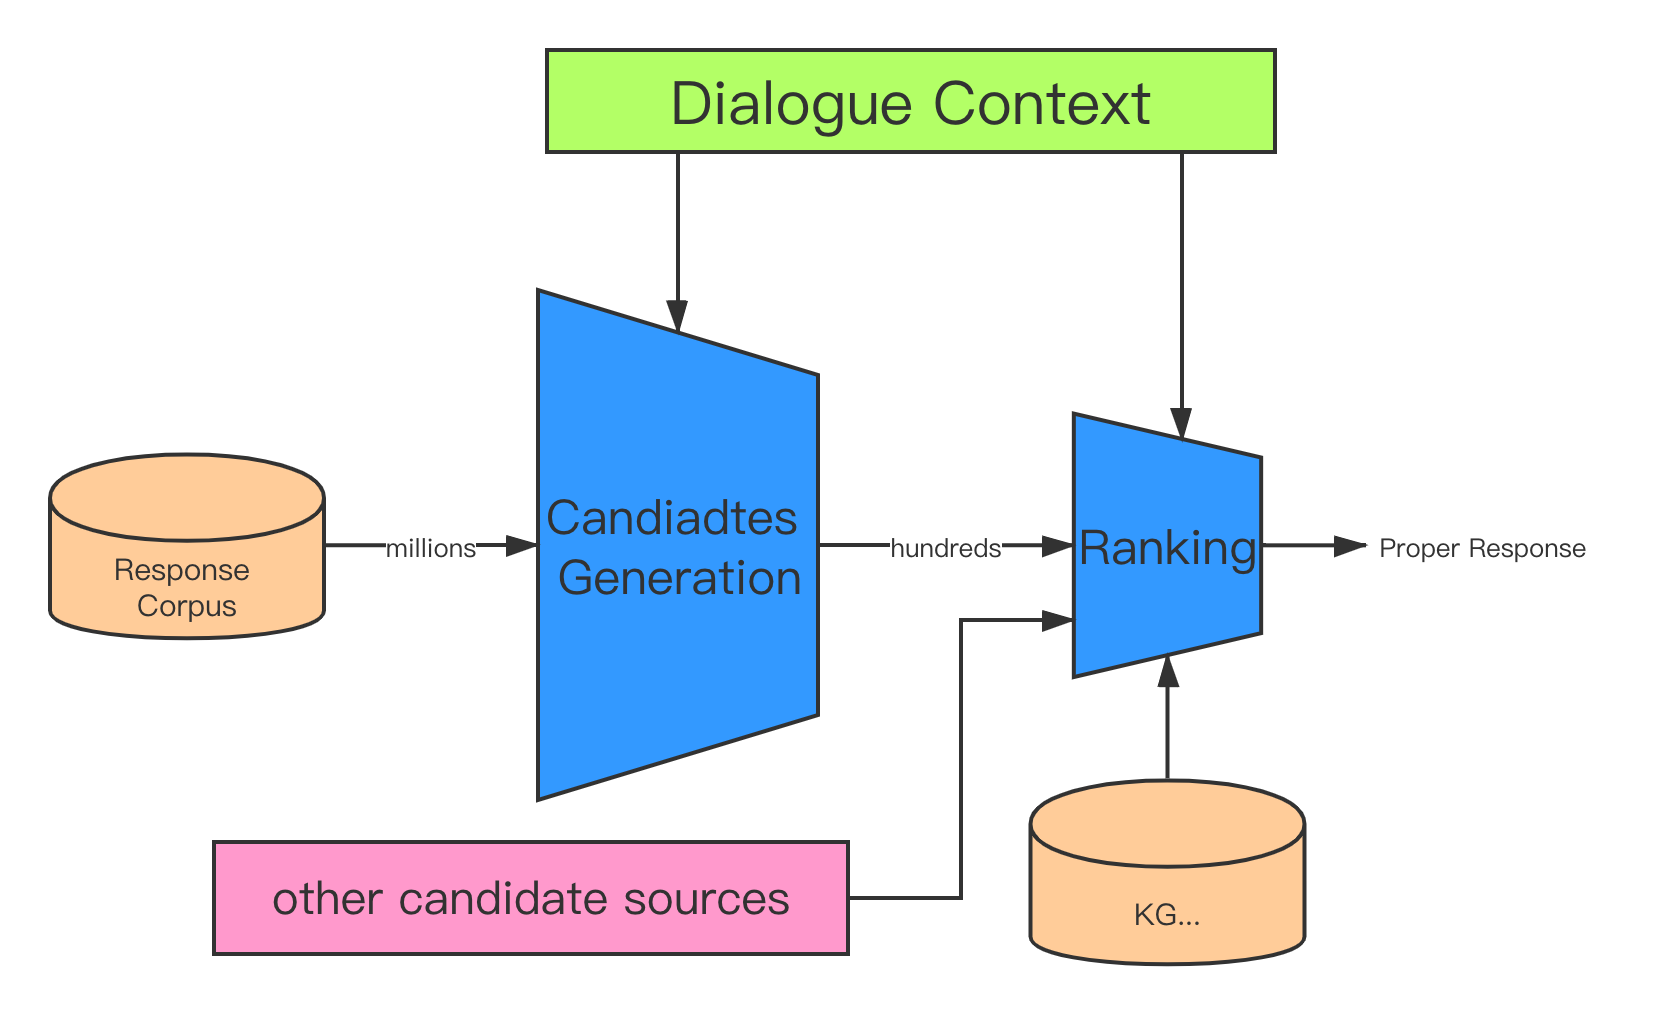
\includegraphics[width=1\linewidth]{arch.png}
    \end{center}
\end{frame}

\begin{frame} {Core Problems in past Initially Immature Architecture}

        \begin{itemize}
            \item Response Corpus has millions responses. It's hard for model to infer within an acceptable time frame. How to reduce the infer time cost?
            \begin{itemize}
                \item How to construct candidates whitelist to reduce the number of candidates?
                \item How to speed up model inferring?
            \end{itemize}
            \item I'm new to training on large scale data. How to make training effective, affordable, and quick?
            \item Training trick on Chinese dataset
        \end{itemize}
        
\end{frame}

% \subsection{Whitelist(Candidates) Generation}
\subsection{Common practice}
\begin{frame}{Common practice for Whitelist Generation}
    \begin{itemize}
        \item Bi-Encoder: created a fix response whitelist
        \begin{itemize}
            \item Frequency-Based Method: select most common agent responses, after accounting for minor variations in capitalization, punctuation, and whitespace.
            \item Clustering-Based Method: encoded all agent responses using response encoder $f_r$ and then used k-means clustering to cluster the responses. Then selected the most common response from each cluster to create the whitelists.
        \end{itemize}
        
        \item Cross-Encoder:  select the top 100 candidates (recall optimization)
        \begin{itemize}
            \item Use Bi-Encoder to select top 100 candidates
            \item Use IR-based methods (TF-IDF match score, cosine similarity with respect to the context)
        \end{itemize}
    \end{itemize}
\end{frame}


\begin{frame}{Comparison Between Whitelist Generations}
    \begin{itemize}
        \item Bi-Encoder: “+” indicates that the true response is added to the whitelist
\begin{tabular}{|c|c|c|c|c|c|}
\hline Whitelist & $\mathbf{R} @ \mathbf{1}$ & $\mathbf{R} @ \mathbf{3}$ & $\mathbf{R} @ \mathbf{5}$ & $\mathbf{R} @ \mathbf{1 0}$ & $\mathbf{B L E U}$ \\
\hline Random 10K+ & 0.252 & 0.400 & 0.472 & 0.560 & 37.71 \\
Frequency 10K+ & 0.257 & 0.389 & 0.455 & 0.544 & 41.34 \\
Clustering 10K+ & 0.230 & 0.376 & 0.447 & 0.541 & 37.59 \\
\hline Random 1K+ & 0.496 & 0.663 & 0.728 & 0.805 & 59.28 \\
Frequency 1K+ & 0.513 & 0.666 & 0.726 & 0.794 & 67.05 \\
Clustering 1K+ & 0.481 & 0.667 & 0.745 & 0.835 & 61.88 \\
\hline \hline Frequency 10K & 0.136 & 0.261 & 0.327 & 0.420 & 30.46 \\
Clustering 10K & 0.164 & 0.292 & 0.360 & 0.457 & 31.47 \\
\hline Frequency 1K & 0.273 & 0.465 & 0.550 & 0.658 & 47.13 \\
Clustering 1K & 0.331 & 0.542 & 0.650 & 0.782 & 49.26 \\
\hline
\end{tabular}
    \end{itemize}
\end{frame}

\begin{frame}{Comparison Between Whitelist Generations}
    \begin{itemize}
        \item Cross-Encoder:
        \begin{tabular}{lllr}
\hline Subtask & Measure & Method1 & Method2 \\
\hline \multirow { Subtask1 } & Recall @ 1 & 0.645 & 0.5262 \\
& Recall @ 10 & 0.902 & 0.7646 \\
& Recall @ 50 & 0.994 & 0.9608 \\
& MRR & 0.735 & 0.6057\\
\hline \multirow { Subtask2 } & Recall @ 1 & 0.067 & 0.1872\\
& Recall@ 10 & 0.185 & 0.3590\\
& Recall @ 50 & 0.266 & 0.6126\\
& MRR & 0.1056 & 0.2513\\
\hline
\end{tabular}
\item Subtask1 has 100 candidates and Subtask2 has 120k candidates
\item Method1 uses Bi-Encoder to select top 100 candidates while Method2 uses IR-based methods
    \end{itemize}
\end{frame}


\subsection{Retrieval Investigation}
\subsubsection{Embedding-based Retrieval}

\begin{frame}{Embedding-based Retrieval in Facebook Search}
    \begin{itemize}
    \item embedding-based retrieval: use embeddings to represent query and documents, and then convert the retrieval problem into a nearest neighbor (NN) search problem in the embedding space.
        \begin{itemize} 
            \item Unified Embedding Model to Learn Query Embedding and Document Embedding
            \item employed Faiss library to quantize the vectors(coarse quantization or  product quantization)
            \item deployed an inverted index based ANN (approximate near neighbor) search algorithms
            % \item a hybrid retrieval framework to integrate \textbf{embedding KNN} and \textbf{Boolean matching} together to score documents for retrieval.
            % \item \textbf{embedding KNN}: employed Faiss library for embedding vector quantization
            % \item \textbf{Boolean matching}: inverted index based retrieval ( Faiss library [9] to quantize the vectors + ANN (approximate near neighbor) search algorithms )
        \end{itemize}
    \end{itemize}
\end{frame}


\subsubsection{Distilling Knowledge}
\begin{frame}{TwinBERT: Distilling Knowledge to Twin-Structured BERT Models for Efficient Retrieval}

\begin{itemize}
    \item To address the latency problem brought by the advanced NLP techniques, this paper proposes a novel language representation model for efficient retrieval(supporting ANN search), called TwinBERT.
    \begin{itemize}
        \item  The model has twin-structured BERT-like encoders to encode the query and document respectively and a crossing layer to combine the two embeddings and produce a similarity score. 
        \item The model was trained following the teacher-student framework. (Knowledge Distillation)
        \item For inference time, the average time cost on CPU over 1,000 random queries was only around 20 milliseconds for scoring 100 documents.
    \end{itemize}
\end{itemize}
    
\end{frame}

\section{Next Work}
\begin{frame}{Next Work}
    \begin{itemize}
        \item Investigating, 之前调研的模型大多以交叉熵为损失函数,需要调研并测试对比学习以及Learn To Rank中pairwise类损失函数,如triplet loss.
        \item Modeling, 模型的Bi-Encoder初步训练, 初步得到response的表示
        \item Serving, 实现PQ和ANN(或者调包),并评估其在对话中召回质量
        \item Optimizing
    \end{itemize}
\end{frame}

\begin{frame}
    \begin{center}
        {\Huge\calligra Thanks!}
    \end{center}
\end{frame}

\section{References}

\begin{frame}[allowframebreaks]
    \bibliography{ref}
    \tiny\bibliographystyle{alpha}
    
    \begin{thebibliography}{10} 
    \bibitem{ref0} Wu Y, Wu W, Xing C, et al. A sequential matching framework for multi-turn response selection in retrieval-based chatbots[J]. Computational Linguistics, 2019, 45(1): 163-197.
    \bibitem{ref1} Swanson K, Yu L, Fox C, et al. Building a Production Model for Retrieval-Based Chatbots[J]. arXiv preprint arXiv:1906.03209, 2019. 
    \bibitem{ref2} Chen Q, Wang W. Sequential attention-based network for noetic end-to-end response selection[J]. arXiv preprint arXiv:1901.02609, 2019.
    \bibitem{ref3} Ganhotra J, Patel S S, Fadnis K. Knowledge-incorporating ESIM models for response selection in retrieval-based dialog systems[J]. arXiv preprint arXiv:1907.05792, 2019.
    \bibitem{ref4} Humeau S, Shuster K, Lachaux M A, et al. Poly-encoders: Transformer architectures and pre-training strategies for fast and accurate multi-sentence scoring[J]. arXiv preprint arXiv:1905.01969, 2019.
    \bibitem{ref5} Huang J T, Sharma A, Sun S, et al. Embedding-based retrieval in facebook search[C]//Proceedings of the 26th ACM SIGKDD International Conference on Knowledge Discovery & Data Mining. 2020: 2553-2561.
    \end{thebibliography}
    % 如果参考文献太多的话,可以像下面这样调整字体:
    % \tiny\bibliographystyle{alpha}
\end{frame}

\section{Appendix(just for reference)}

\begin{frame}{Dataset Ubuntu Dialogue Corpus v1.0}
    \begin{itemize}
        \item The new Ubuntu Dialogue Corpus consists of
almost one million two-person conversations extracted from the Ubuntu chat logs1
, used to receive
technical support for various Ubuntu-related problems. 

    \end{itemize}
    \begin{center} \tiny
        \begin{tabular}{|c|c|}
\hline # dialogues (human-human) & 930,000 \\
\hline # utterances (in total) & 7,100,000 \\
\hline # words (in total) & 100,000,000 \\
\hline Min. # turns per dialogue & 3 \\
\hline Avg. # turns per dialogue & 7.71 \\
\hline Avg. # words per utterance & 10.34 \\
\hline Median conversation length (min) & 6 \\
\hline
\end{tabular}

\begin{tabular}{|l|l|c|}
\hline Context & Response & Flag \\
\hline well, can I move the drives? \_\_EOS\_\_ ah not like that & I guess I could just get an enclosure and copy via USB & 1 \\
\hline Well, can I move the drives? \_\_EOS\_\_ & you can use "ps ax" and "kill (PID #)" & 0 \\
\hline
\end{tabular}
    \end{center}
    
\end{frame}

\begin{frame}{Dataset DSTC7-Ubuntu}
    \begin{itemize}
        \item Subtask 1\ 100 candidates, including 1 correct option.
\item Subtask 2\ 120,000 candidates, including 1 correct option (Ubuntu data only).

\item Subtask 3\ 100 candidates, including $1-5$ correct options that are paraphrases (Advising data only).
\item Subtask 4\ 100 candidates, including $0-1$ correct options.
\item Subtask 5 The same as subtask $1,$ but with access to external information.
    \end{itemize}
    
    \begin{center}\tiny
        \begin{tabular}{lrr}
\hline Property & Advising & Ubuntu \\
\hline \hline Dialogues & 500 & 135,078 \\
Utterances / Dialogue & 18.6 & 10.0 \\
Tokens / Utterance & 9.6 & 9.9 \\
Utterances / Unique utterances & 4.4 & 1.1 \\
Tokens / Unique tokens & 10.5 & 22.9 \\
\hline
\end{tabular}
    \end{center}
\end{frame}

\begin{frame}{Dataset Persona-Chat}
The data collection consists of three stages:

(i) \textbf{Personas}: we crowdsource a set of 1155 possible personas, each consisting of at least 5 profile sentences, setting aside 100 never seen before personas for validation, and 100 for test.


(ii) \textbf{Revised personas}: to avoid modeling that takes advantage of trivial word overlap, we crowdsource additional rewritten sets of the same 1155 personas, with related sentences that are rephrases, generalizations or specializations


(iii) \textbf{Persona chat}: we pair two Turkers and assign them each a random (original) persona from the pool, and ask them to chat. This resulted in a dataset of 162,064 utterances over 10,907 dialogs, 15,602 utterances ($1000$ dialogs) of which are set aside for validation, and 15,024 utterances ($968$ dialogs) for test.
\end{frame}

\begin{frame}{Dataset Persona-Chat}
Example:
\begin{center}\tiny
\begin{tabular}{l|l}
\hline Persona 1 & Persona 2 \\
\hline I like to ski & I am an artist \\
My wife does not like me anymore & I have four children \\
I have went to Mexico 4 times this year & I recently got a cat \\
I hate Mexican food & I enjoy walking for exercise \\
I like to eat cheetos & I love watching Game of Thrones \\
\hline
\end{tabular}
\end{center}
\tiny
[PERSON 1:] Hi

[PERSON 2:] Hello ! How are you today ? 

[PERSON 1:] I am good thank you , how are you. 

[PERSON 2:] Great, thanks ! My children and I were just about to watch Game of Thrones. 

[PERSON 1:] Nice ! How old are your children? 

[PERSON 2:] I have four that range in age from 10 to $21 .$ You? 

[PERSON 1:] I do not have children at the moment. 

[PERSON 2:] That just means you get to keep all the popcorn for yourself. 

[PERSON 1:] And Cheetos at the moment! 

[PERSON 2:] Good choice. Do you watch Game of Thrones? 

[PERSON 1:] No, I do not have much time for TV. 

[PERSON 2:] I usually spend my time painting: but, I love the show.

\end{frame}

\begin{frame}{Dataset Reddit}
Reddit conversations are threaded. Each post may have multiple top-level comments, and every comment may have multiple children comments written in response. In processing, each Reddit thread is used to generate a set of examples. 

The data from 2015 to 2018 inclusive consists of
3,680,746,776 comments, in 256,095,216 threads.
In total, 727,013,715 Tensorflow examples are created from this data.
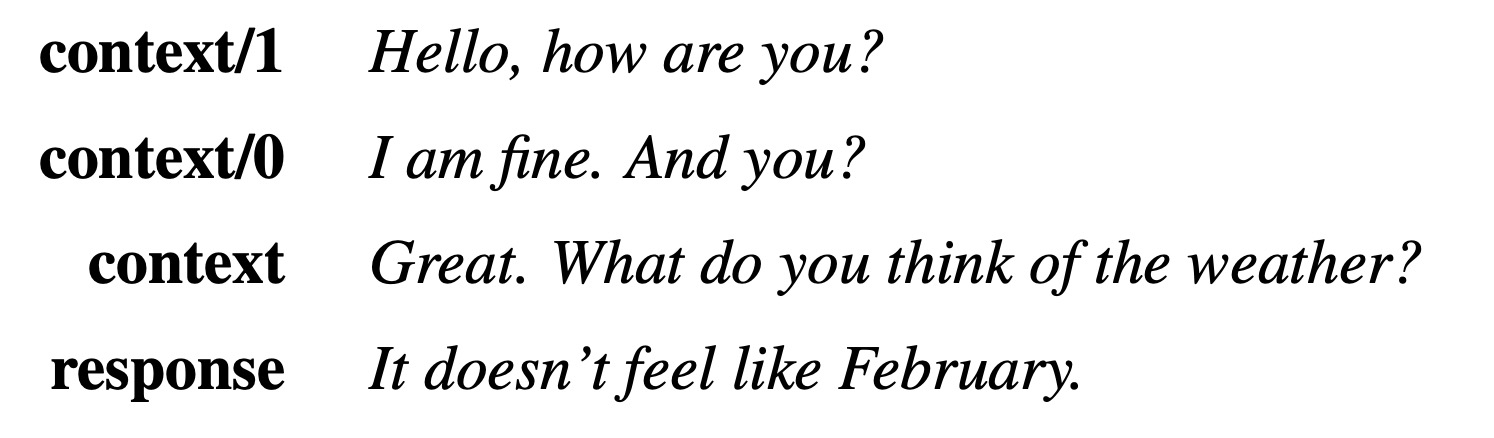
\includegraphics[width=0.5\linewidth]{reddit.png}
\end{frame}


\begin{frame}{Dataset Douban}
 open domain conversation
 
 \begin{tabular}{c|c|c|c}
\hline & train & val & test \\
\hline # context-response pairs & $1 \mathrm{M}$ & $50 \mathrm{k}$ & $10 \mathrm{k}$ \\
\hline # candidates per context & 2 & 2 & 10 \\
\hline # positive candidates per context & 1 & 1 & 1.18 \\
\hline Min. # turns per context & 3 & 3 & 3 \\
\hline Max. # turns per context & 98 & 91 & 45 \\
\hline Avg. # turns per context & 6.69 & 6.75 & 6.45 \\
\hline Avg. # words per utterance & 18.56 & 18.50 & 20.74 \\
\hline
\end{tabular}

\end{frame}

\begin{frame}{Dataset LCCC}
 The quality of our dataset is ensured by a rigorous data cleaning pipeline, which
is built based on a set of rules and a classifier that is trained on manually annotated 110K dialogue pairs
    \begin{center}\footnotesize
        \begin{tabular}{l|c|c|c|c} 
\hline & Single-Turn & Multi-Turn & Single-Turn& Multi-Turn \\
\hline Raw dialogs & 52,708,95.5 & 26,749,365 & 63,251,887 & 28,189,952 \\
Cleaned dialogs & 3,354,382 & 3,466,607 & 7,273,804 & 4,733,955 \\
Utterances & 6,708,554 & 13,365,268 & 14,547,608 & 18,341,167 \\
Characters & 68,559,727 & 163,690,614 & 162,301,556 & 217,776,649 \\
Vocabulary size & 372,063 & 666,931 & 662,514 & 690,027 \\
Avg. words & 6.79 & 8.36 & 7.45 & 8.14 \\
Avg. turns & 2 & 3.86 & 2 & 3.87 \\
\hline
\end{tabular}
Statistics of LCCC-base (left) and LCCC-large (right)
    \end{center}
    
\end{frame}

\begin{frame}{Poly-Encoder}
    Motivation: improve both the quality and speed
    \begin{itemize}
        \item Pre-trained two transformer models \textbf{from scratch} with the same architecture and dimension as BERT-base. 
        \begin{itemize}
            \item One uses 150 million of [INPUT, LABEL] extracted from Wikipedia and Toronto Books Corpus, while the other is trained on 174 million extracted from Reddit. 
            \item Pre-training strategy: a \textbf{masked language model} (MLM) task + a \textbf{next-utterance prediction} task(an utterance can be composed of several sentences!)
        \end{itemize}
        
        % \item The Poly-encoder architecture:
        % \begin{center}
        %     % \includegraphics[]{}
        %     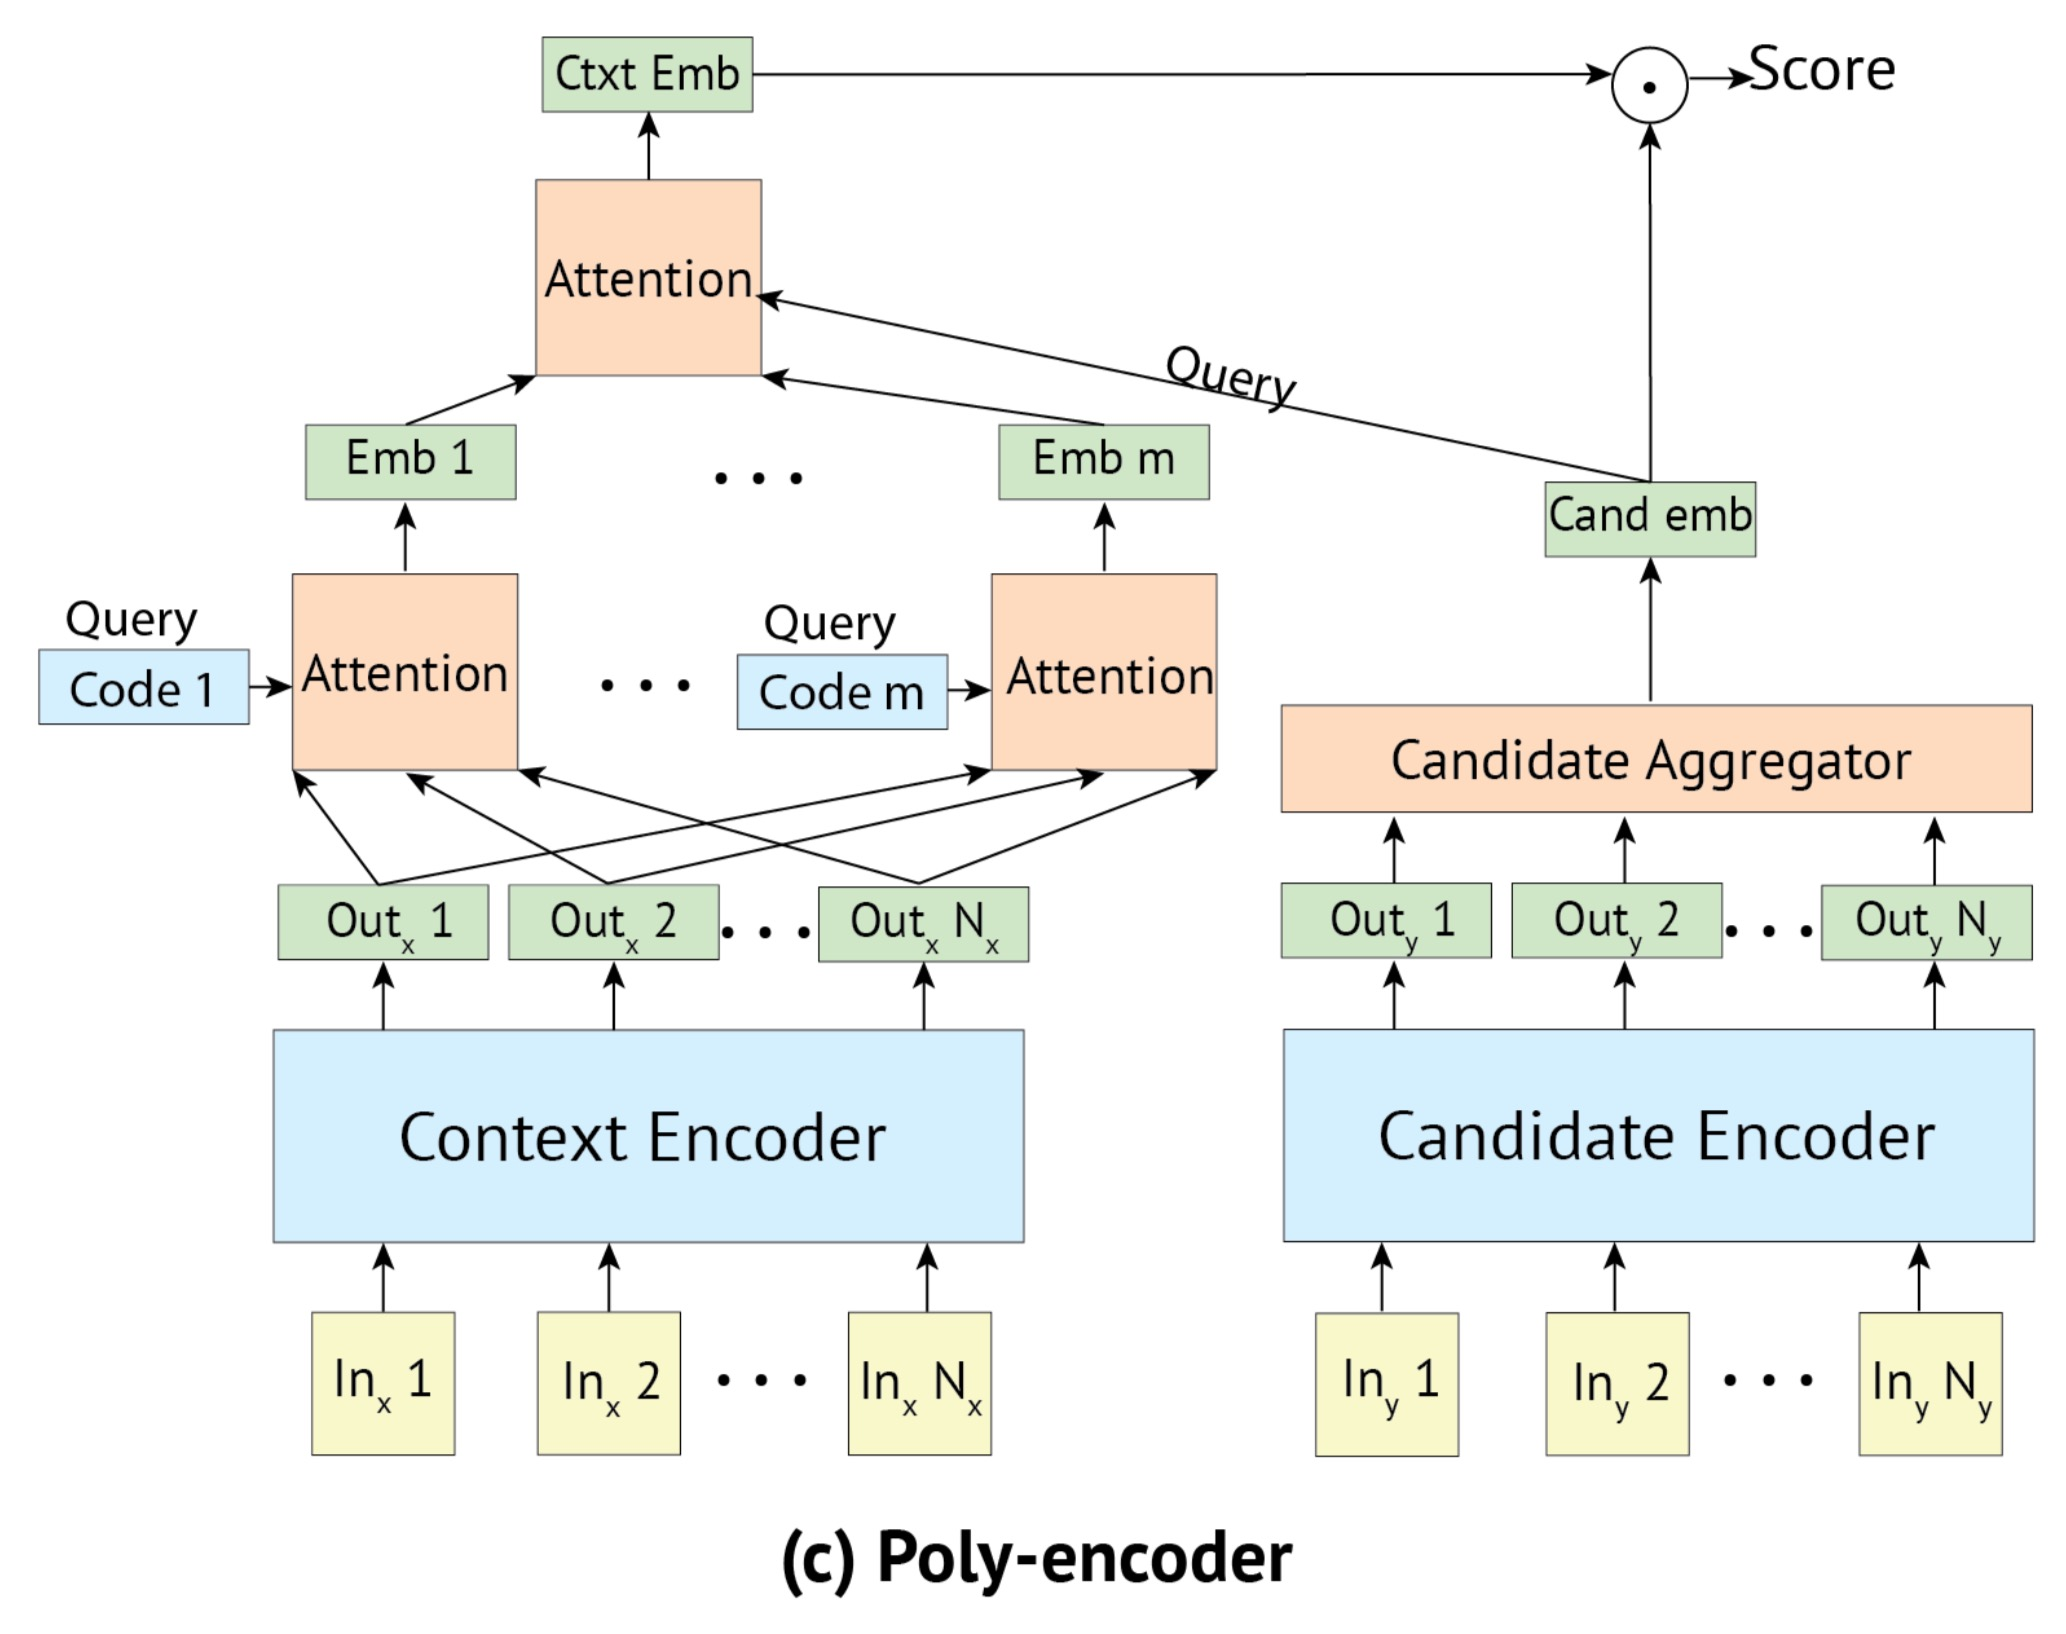
\includegraphics[width=0.9\linewidth]{poly-encoder.png}
        % \end{center}
       
    \end{itemize}
\end{frame}

\begin{frame}{Poly-Encoder}
    \begin{itemize}
        \item The Poly-encoder architecture:
        \begin{center}
            % \includegraphics[]{}
            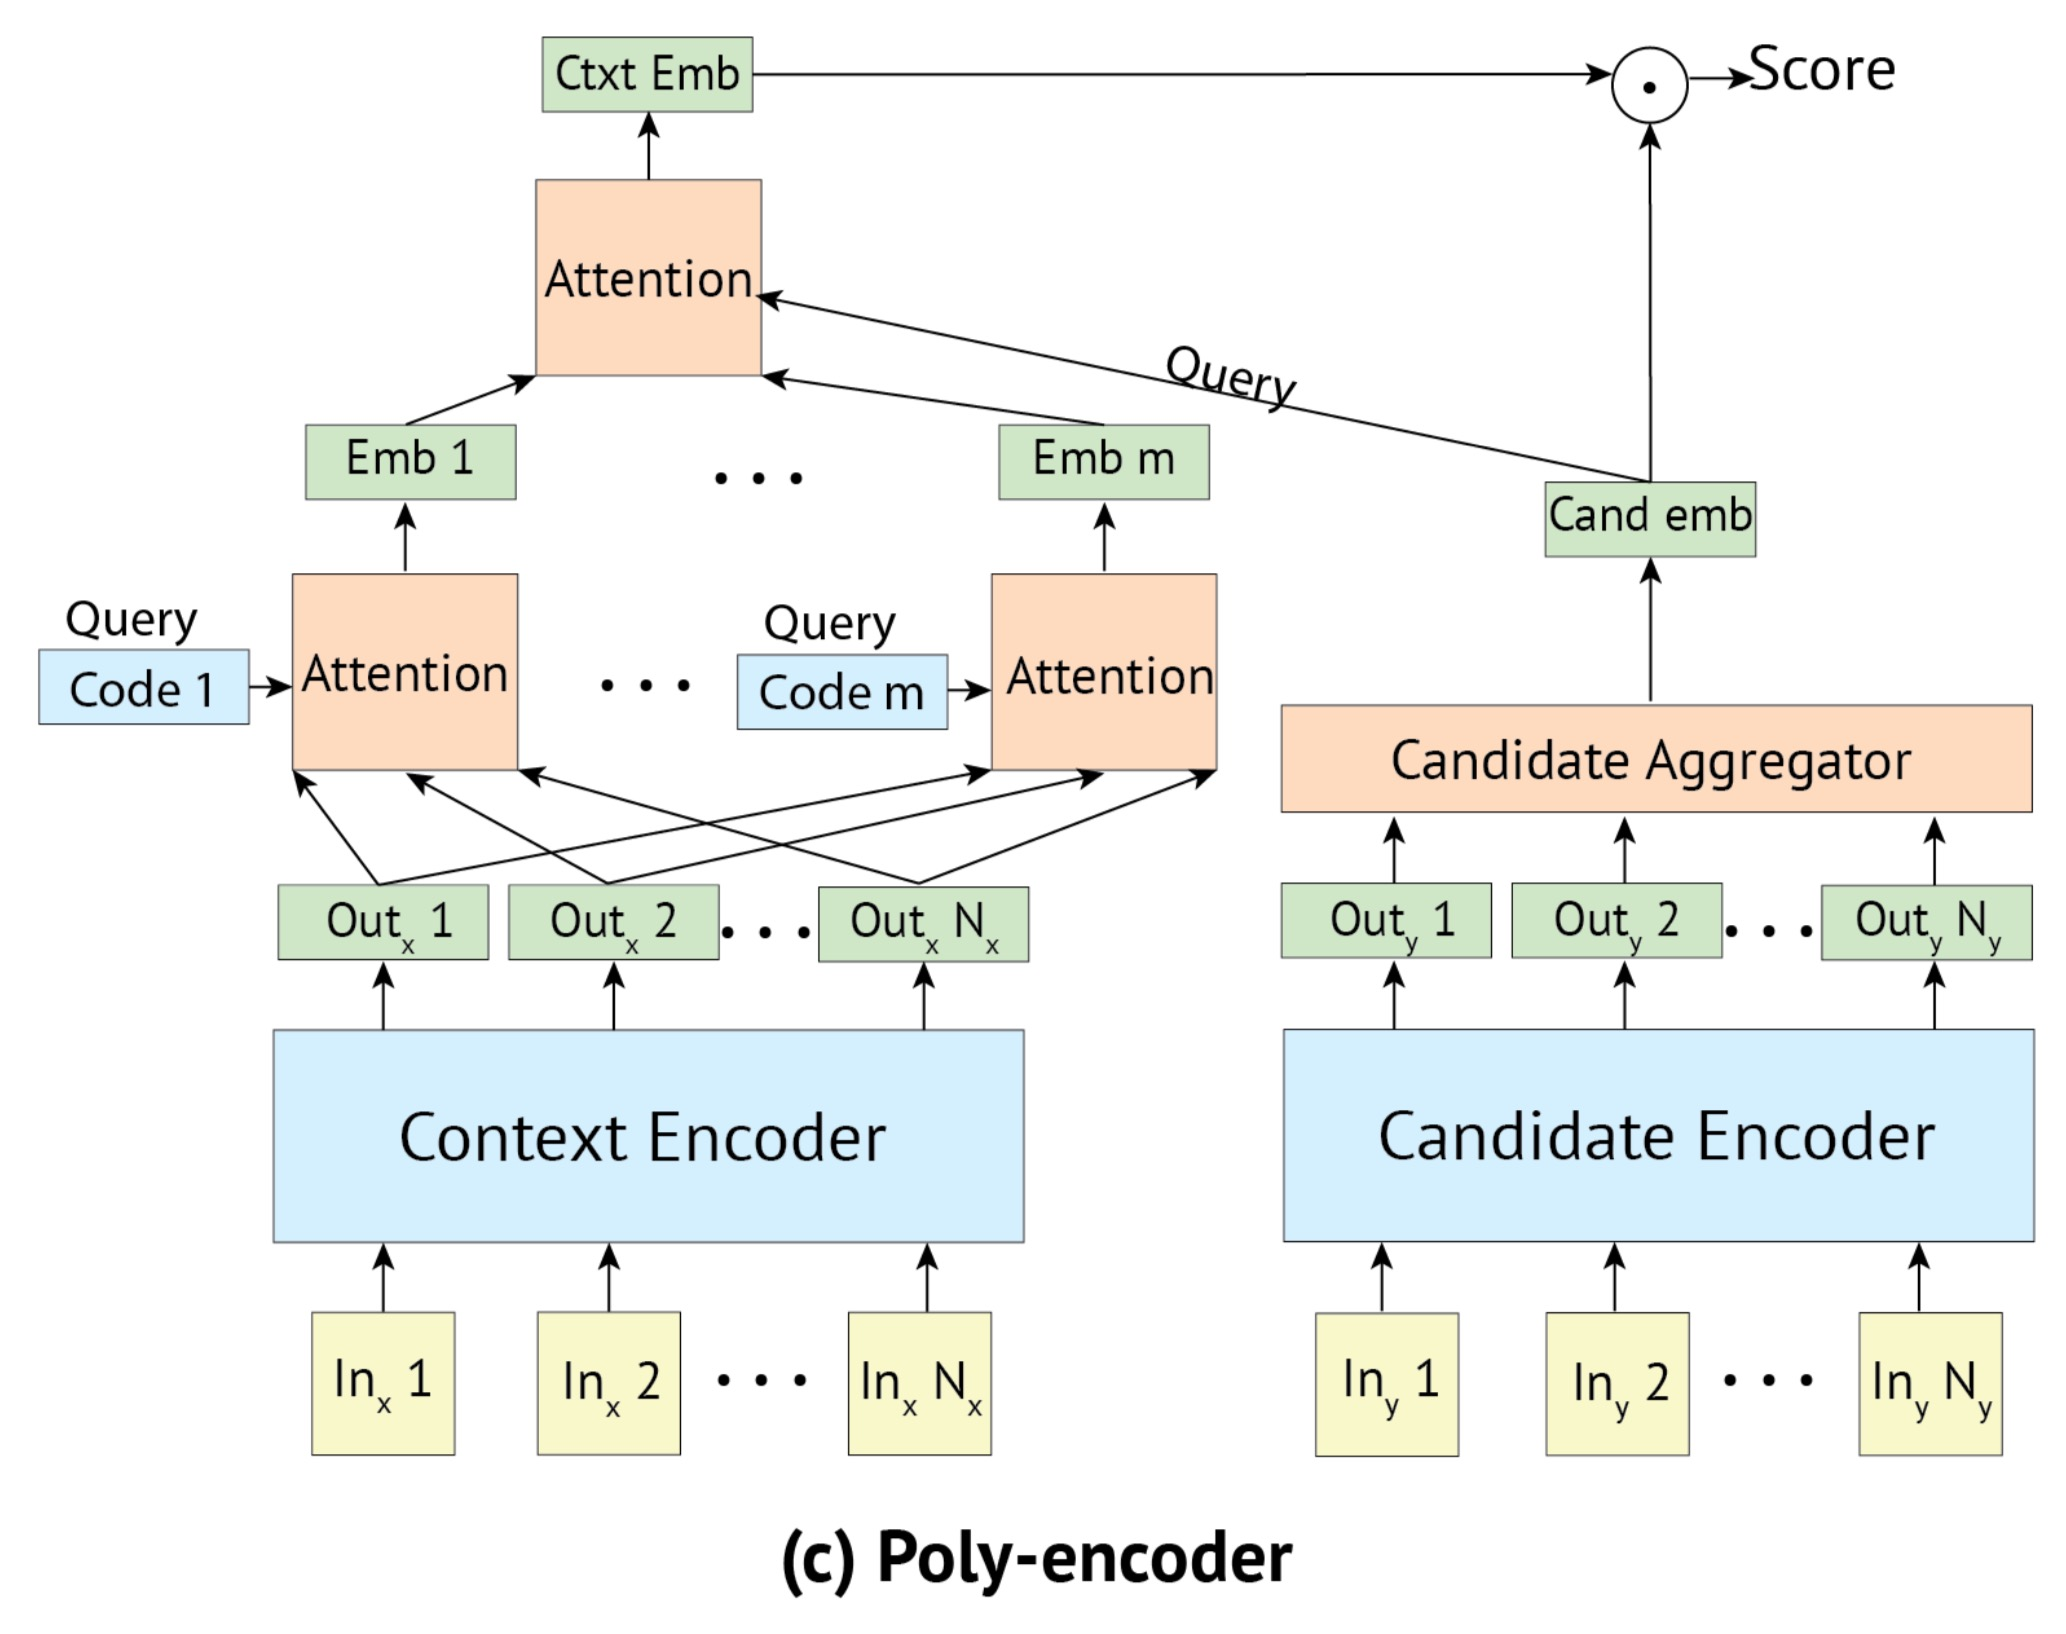
\includegraphics[width=0.9\linewidth]{poly-encoder.png}
        \end{center}
       
    \end{itemize}
\end{frame}

\begin{frame}{Poly-Encoder}
    The input context, which is typically much longer than a candidate, is represented with m vectors $(y^1_{ctxt}..y^m_{ctxt})$ instead of just one as in the Bi-encoder, where m will influence the inference speed.
    
    \begin{center}
        $y_{c t x t}^{i}=\sum_{j} w_{j}^{c_{i}} h_{j} \quad$ 
    
    where $\quad\left(w_{1}^{c_{i}}, \ldots, w_{N}^{c_{i}}\right)=\operatorname{softmax}\left(c_{i} \cdot h_{1}, . ., c_{i} \cdot h_{N}\right)$
    \end{center}
    The m context codes$(c_1, ..., c_m)$ are randomly initialized, and learnt during finetuning.
    
    Finally, given m global context features, using $y_{cand_i}$ as the query: (Huge Cost)
    \begin{center}
        $y_{c t x t}=\sum_{i} w_{i} y_{c t x t}^{i} \quad$ where $\quad\left(w_{1}, . ., w_{m}\right)=\operatorname{softmax}\left(y_{c a n d_{i}} \cdot y_{c t x t}^{1}, . ., y_{c a n d_{i}} \cdot y_{c t x t}^{m}\right)$
    \end{center}
    
\end{frame}

\begin{frame}{Poly-Encoder}
    Test performance of Bi-, Poly- and Cross-encoders on our selected tasks.
    (Pre-training on Reddit)
    \begin{center}
    \footnotesize

    \begin{tabular}{|l|c|c|c|c|c|}
        \hline Dataset & ConvAI2 & \multicolumn{2}{|c|} { DSTC 7} & \multicolumn{2}{c|} { Ubuntu v2 } \\
        \hline split & test & \multicolumn{2}{|c|} { test } & \multicolumn{2}{c|} { test } \\
        \hline metric & R @ 1/20 & R@1/100 & MRR & R @ 1/10 & MRR \\
        \hline
        
        \hline Bi-encoder & $84.8 \pm 0.1$ & $70.9 \pm 0.5$ & $78.1 \pm 0.3$ & $83.6 \pm 0.7$ & $90.1 \pm 0.4$ \\
        \hline Poly-encoder 16 & $86.3 \pm 0.3$ & $71.6 \pm 0.6$ & $78.4 \pm 0.4$ & $86.0 \pm 0.1$ & $91.5 \pm 0.1$ \\
        \hline Poly-encoder 64 & $86.5 \pm 0.2$ & $71.2 \pm 0.8$ & $78.2 \pm 0.7$ & $85.9 \pm 0.1$ & $91.5 \pm 0.1$ \\
        \hline Poly-encoder 360 & $86.8 \pm 0.1$ & $71.4 \pm 1.0$ & $78.3 \pm 0.7$ & $85.9 \pm 0.1$ & $91.5 \pm 0.0$ \\
        \hline Cross-encoder & $\mathbf{8 7 . 9 \pm 0 . 2}$ & $\mathbf{7 1 . 7 \pm 0 . 3}$ & $\mathbf{7 9 . 0 \pm 0 . 2}$ & $\mathbf{8 6 . 5 \pm 0 . 1}$ & $\mathbf{9 1 . 9 \pm 0 . 0}$ \\
        \hline
        
    \end{tabular}
    
  \end{center}
\end{frame}


\begin{frame}{Poly-Encoder}
    Average time in milliseconds to predict the next dialogue utterance from C possible candidates on ConvAI2. * are inferred.
    
    \begin{center}
        

    
    \begin{tabular}{|c|c|c|c|c|}
\hline & \multicolumn{4}{|c|} { Scoring time (ms) } \\
\hline & \multicolumn{2}{|c|} { CPU } & \multicolumn{2}{c|} { GPU } \\
\hline Candidates & $1 \mathrm{k}$ & $100 \mathrm{k}$ & $1 \mathrm{k}$ & $100 \mathrm{k}$ \\
\hline \hline Bi-encoder & 115 & 160 & 19 & 22 \\
\hline Poly-encoder 16 & 122 & 678 & 18 & 38 \\
\hline Poly-encoder 64 & 126 & 692 & 23 & 46 \\
\hline Poly-encoder 360 & 160 & 837 & 57 & 88 \\
\hline Cross-encoder & $21.7 \mathrm{k}$ & $2.2 \mathrm{M}^{*}$ & $2.6 \mathrm{k}$ & $266 \mathrm{k}^{*}$ \\
\hline
\end{tabular}
    \end{center}
CPU computations were run on an 80 core Intel Xeon processor CPU E5-2698. GPU computations were run on a single Nvidia Quadro GP100 using cuda 10.0 and cudnn 7.4.
\end{frame}


\begin{frame}{ConveRT}
Motivation: a pretraining framework for conversational tasks satisfying: effective, affordable, and quick to train
    \begin{itemize}
        \item Randomly sample 10M sentences from Reddit to run \textbf{subword} tokenization ,get a vocabulary of 31,476 tokens.
        \item Pretraining on Reddit Data.
        \item Lots of tricks in training: two positional encoding, maximum relative attention in Transformer, square-root-of-N reduction...
        \item Quantization: all embedding parameters are represented using only 8 bits, and other network parameters with just 16 bits
    \end{itemize}
\end{frame}

\begin{frame}{ConveRT}
\begin{figure}[htbp]
\centering
\begin{minipage}[t]{0.48\textwidth}
\centering
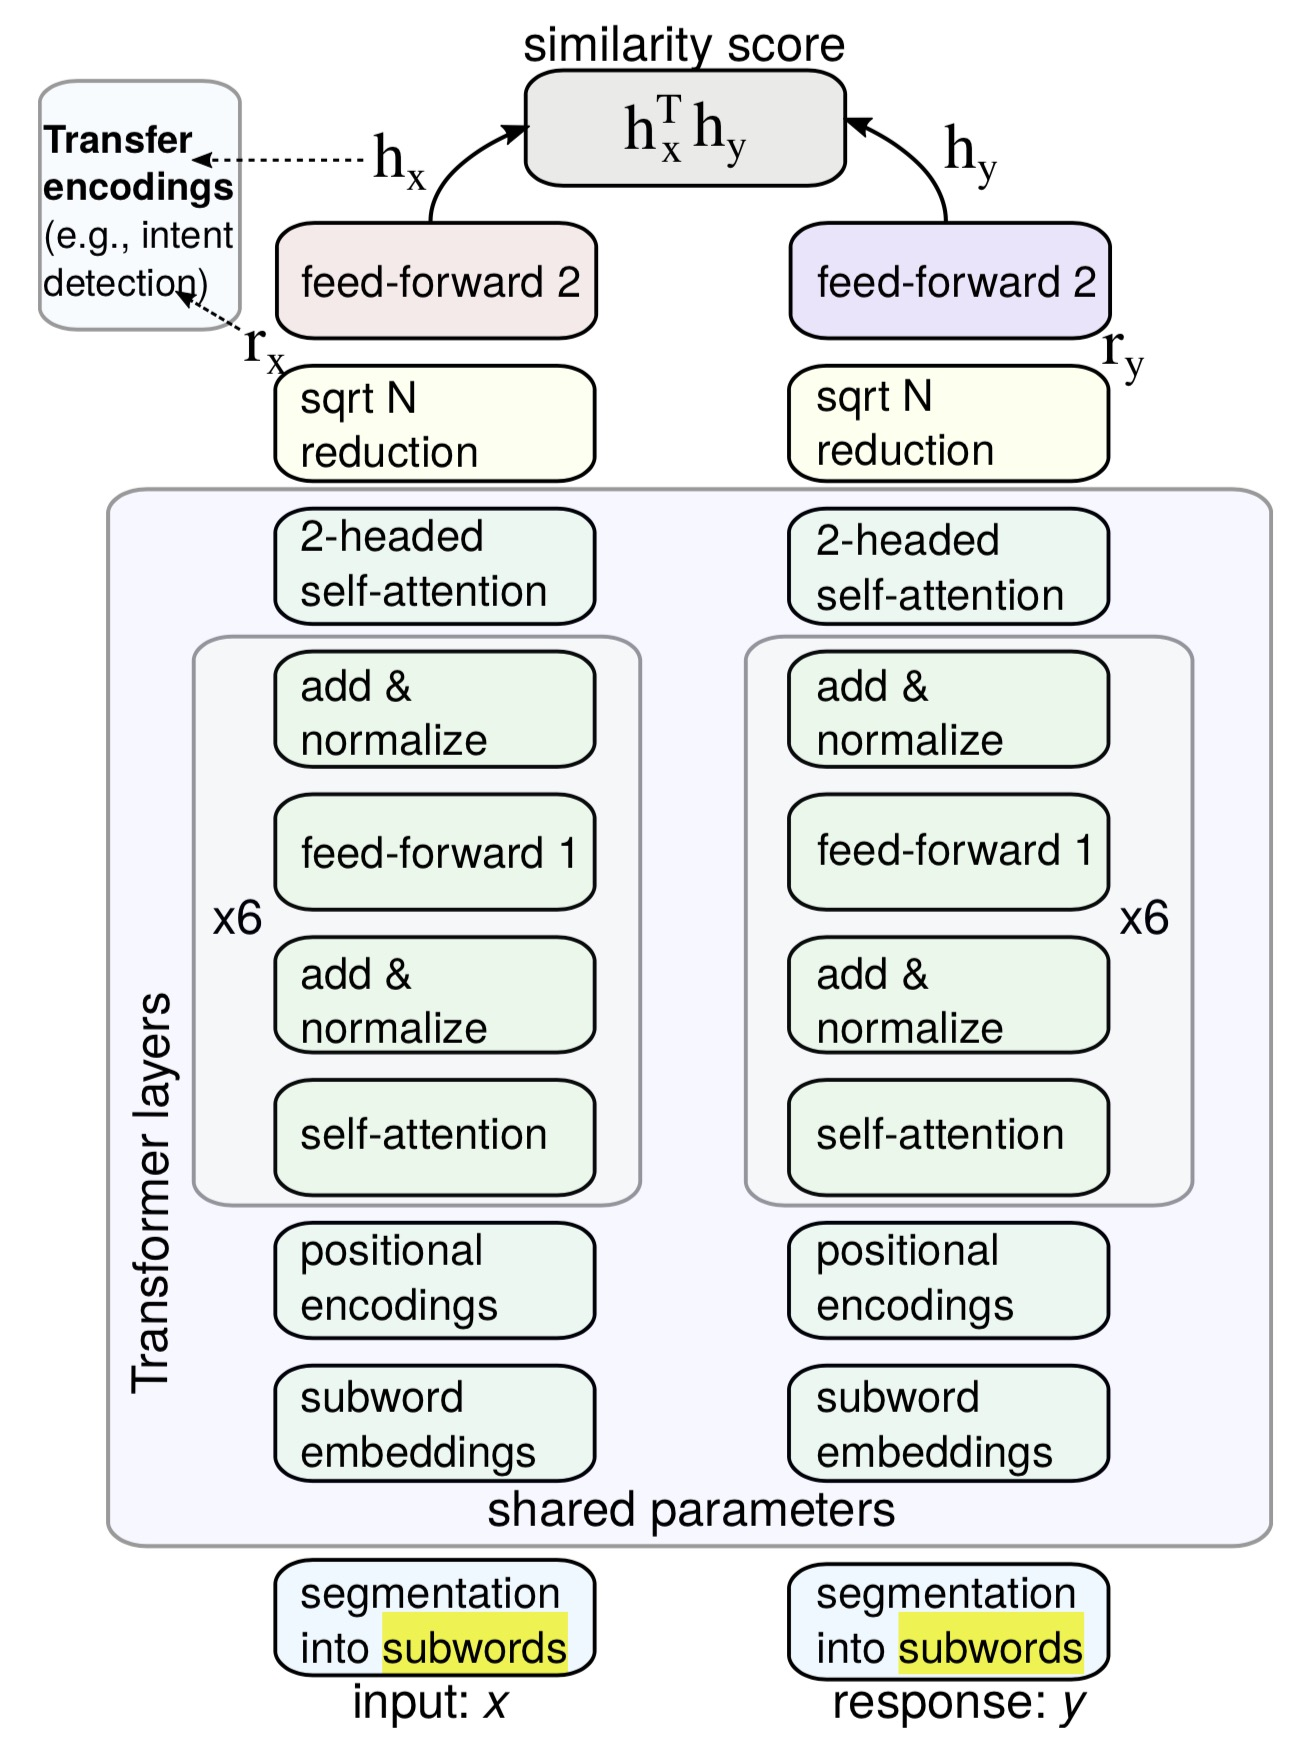
\includegraphics[width=4.5cm]{ConveRT1.png}
\caption{Single-context ConveRT}
\end{minipage}
\begin{minipage}[t]{0.48\textwidth}
\centering
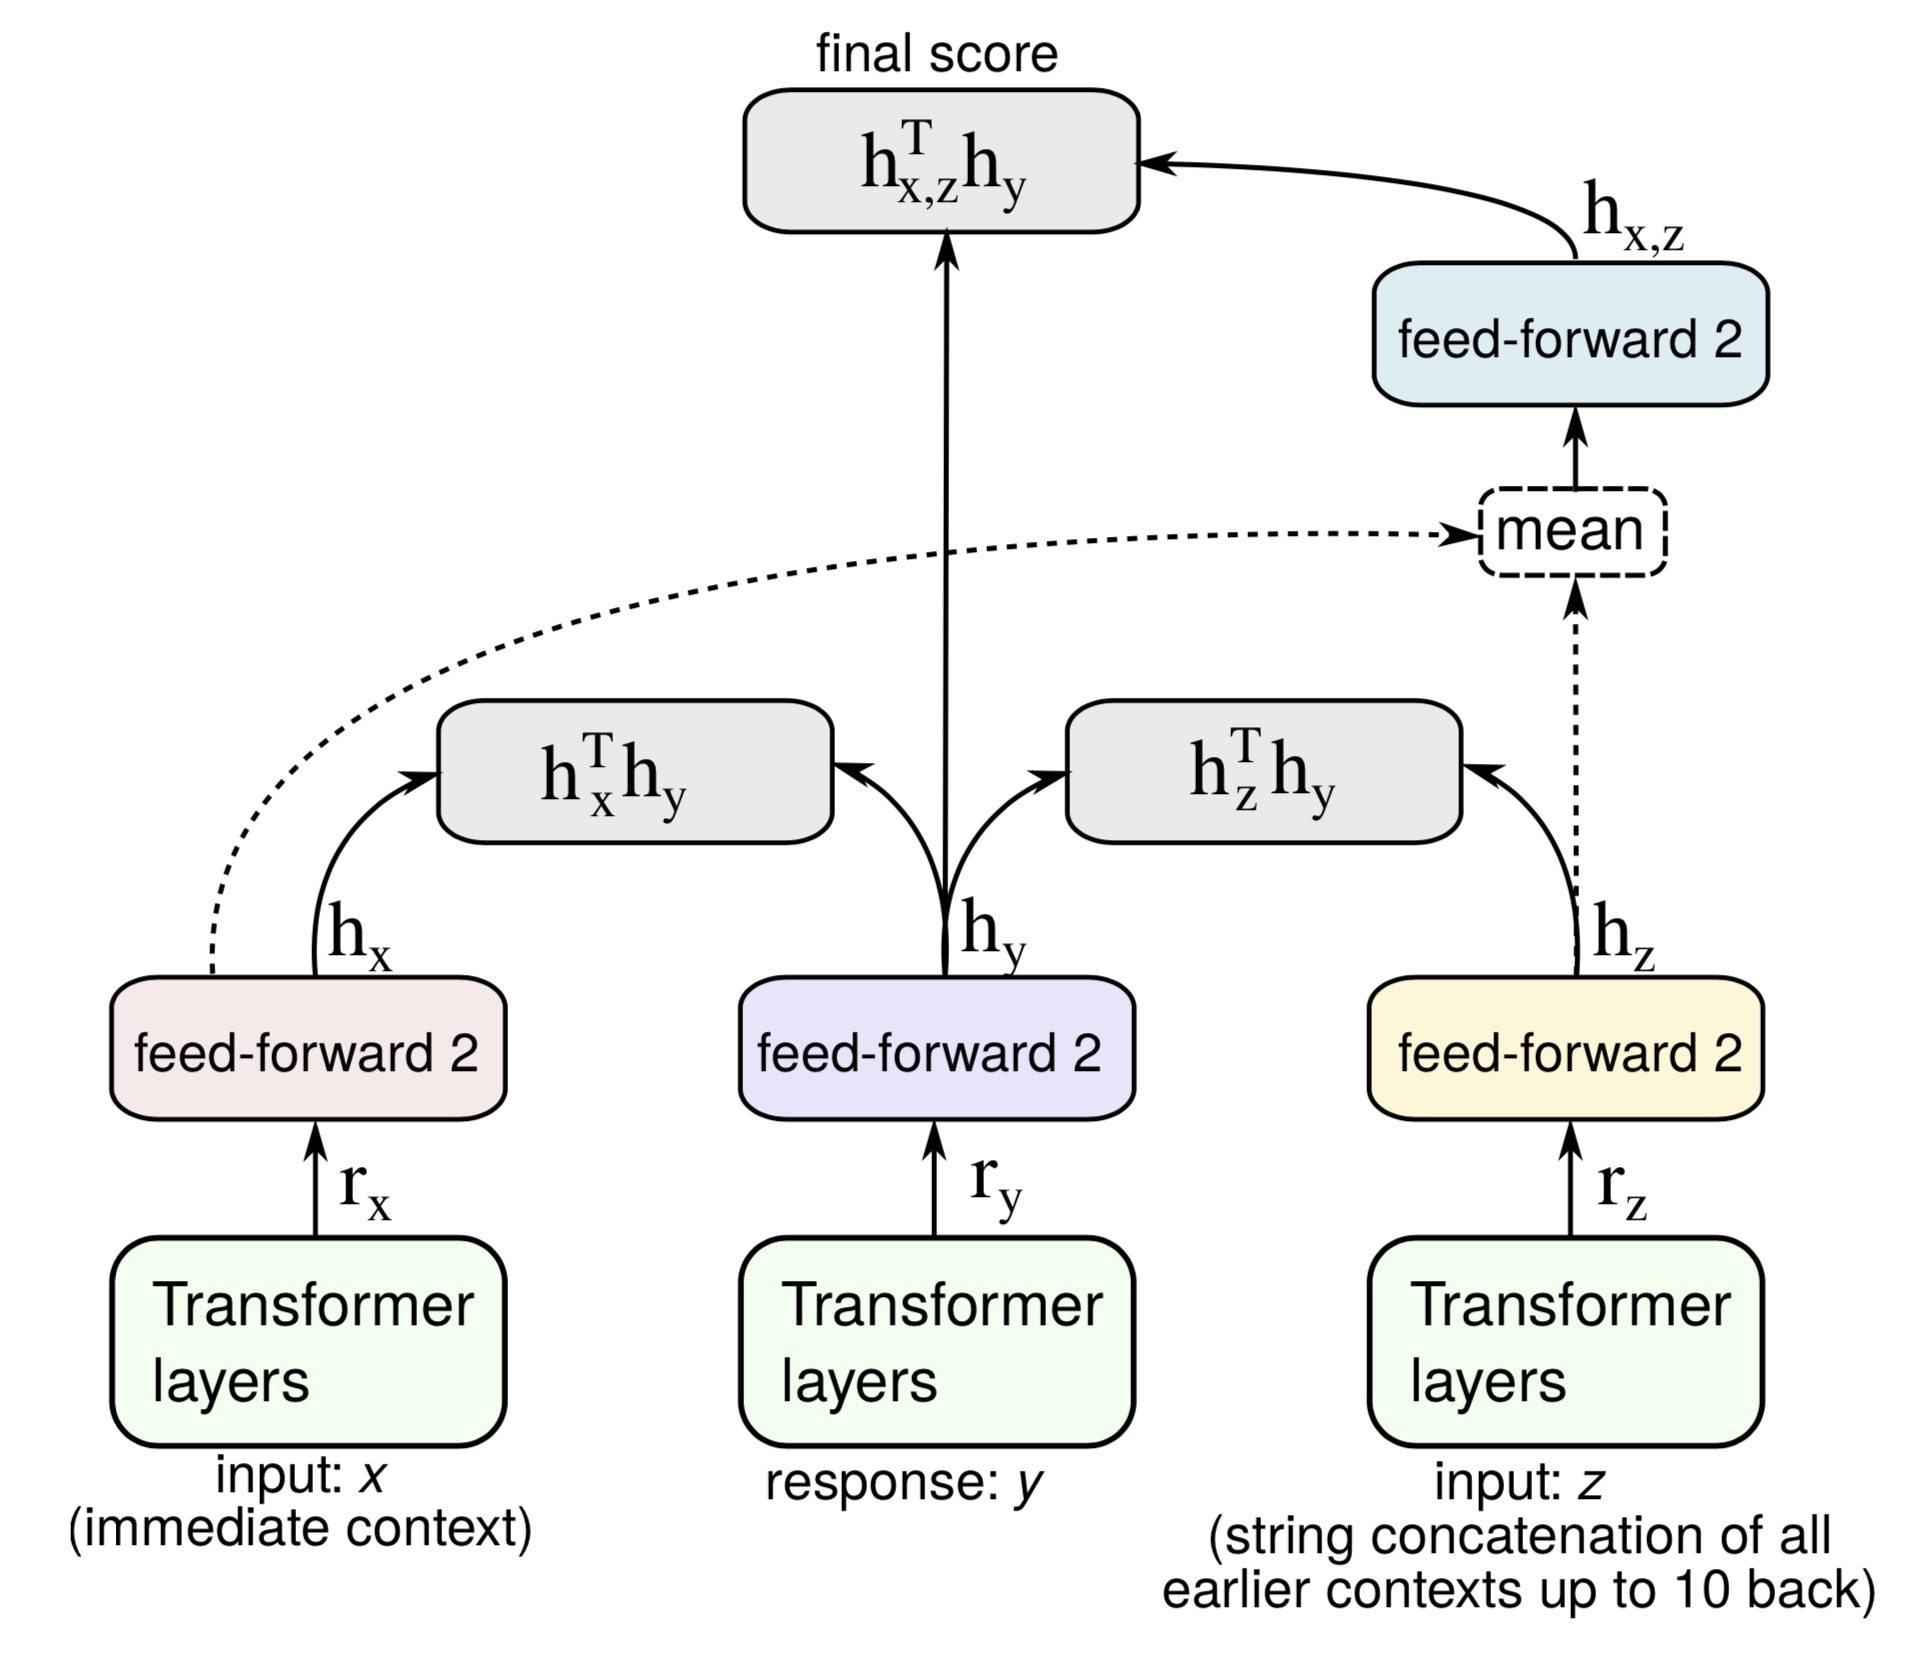
\includegraphics[width=4.5cm]{ConveRT2.png}
\caption{Multi-context ConveRT}
\end{minipage}
\end{figure}

\end{frame}

\begin{frame}{ConveRT}
Results:
\begin{center}\footnotesize
\begin{tabular}{lcc} 
\hline & Reddit & AmazonQA \\
\cline { 2 - 3 } TF-IDF & 26.4 & 51.8 \\
USE-LARGE-MAP & 47.7 & 61.9 \\
BERT-LARGE-MAP & 24.0 & 44.1 \\
USE-QA-MAP & 46.6 & 70.7 \\
POLYAI-DUAL & 61.3 & 71.3 \\
\hline ConveRT (single-context) & 68.2 & 84.3 \\
ConveRT (multi-context) & $\mathbf{7 1 . 8}$ & $-$ \\
\hline
\end{tabular}
\end{center}

\begin{center}\footnotesize

    \begin{tabular}{lcc}
\hline & $\mathbf{R}_{100} @ 1$ & MRR \\
\cline { 2 - 3 } Best DSTC7 System & 64.5 & 73.5 \\
GPT* & 48.9 & 59.5 \\
BERT* & 53.0 & 63.2 \\
Bi-encoder (Humeau et al., 2020) & 70.9 & 78.1 \\
\hline ConveRT (single-context) & 38.2 & 49.2 \\
ConveRT (multi-context) & $\mathbf{7 1 . 2}$ & $\mathbf{7 8 . 8}$ \\
\hline
\end{tabular}
\end{center}

\end{frame}

\begin{frame}{ConveRT}
Comparison of the proposed compact dual-encoder architecture for response selection to existing public standard sentence embedding models.
\begin{center} \tiny

    \begin{tabular}{lcccc}
\hline & Embedding param & Network param & Total size & Size after quantization \\
\hline USE (Cer et al., 2018) & $256 \mathrm{M}$ & $2 \mathrm{M}$ & $1033 \mathrm{MB}$ & $261 \mathrm{MB}^{*}$ \\
BERT-BASE (Devlin et al., 2019) & $23 \mathrm{M}$ & $86 \mathrm{M}$ & $438 \mathrm{MB}$ & $196 \mathrm{MB} * / 110 \mathrm{MB} * *$ \\
BERT-LARGE (Devlin et al., 2019) & $31 \mathrm{M}$ & $304 \mathrm{M}$ & $1341 \mathrm{MB}$ & $639 \mathrm{MB} * / 336 \mathrm{MB} * *$ \\
GPT-2 (Radford et al., 2019) & $80 \mathrm{M}$ & $1462 \mathrm{M}$ & $6168 \mathrm{MB}$ & $3004 \mathrm{MB} *$ \\
POLYAI-DUAL & $104 \mathrm{M}$ & $7 \mathrm{M}$ & $444 \mathrm{MB}$ & $118 \mathrm{MB}$ \\
\hline ConveRT (this work) & $16 \mathrm{M}$ & $13 \mathrm{M}$ & $116 \mathrm{MB}$ & $\mathbf{5 9 M B}$ \\
\hline
\end{tabular}
    
\end{center}
\end{frame}

\begin{frame}{Bert-SL}
Motivation: Existing studies focus on building a context-response matching model, \textbf{overlook many potential training signals} beneficial for context understanding and better features for response prediction.

Propose \textbf{four self-supervised auxiliary tasks}, jointly train the PLM-based response selection model.
    \begin{itemize}
        \item next session prediction
        \item utterance restoration
        \item incoherence detection
        \item consistency discrimination
    \end{itemize}
\end{frame}


\begin{frame}{Bert-SL}
            \begin{center}
            % \includegraphics[]{}
            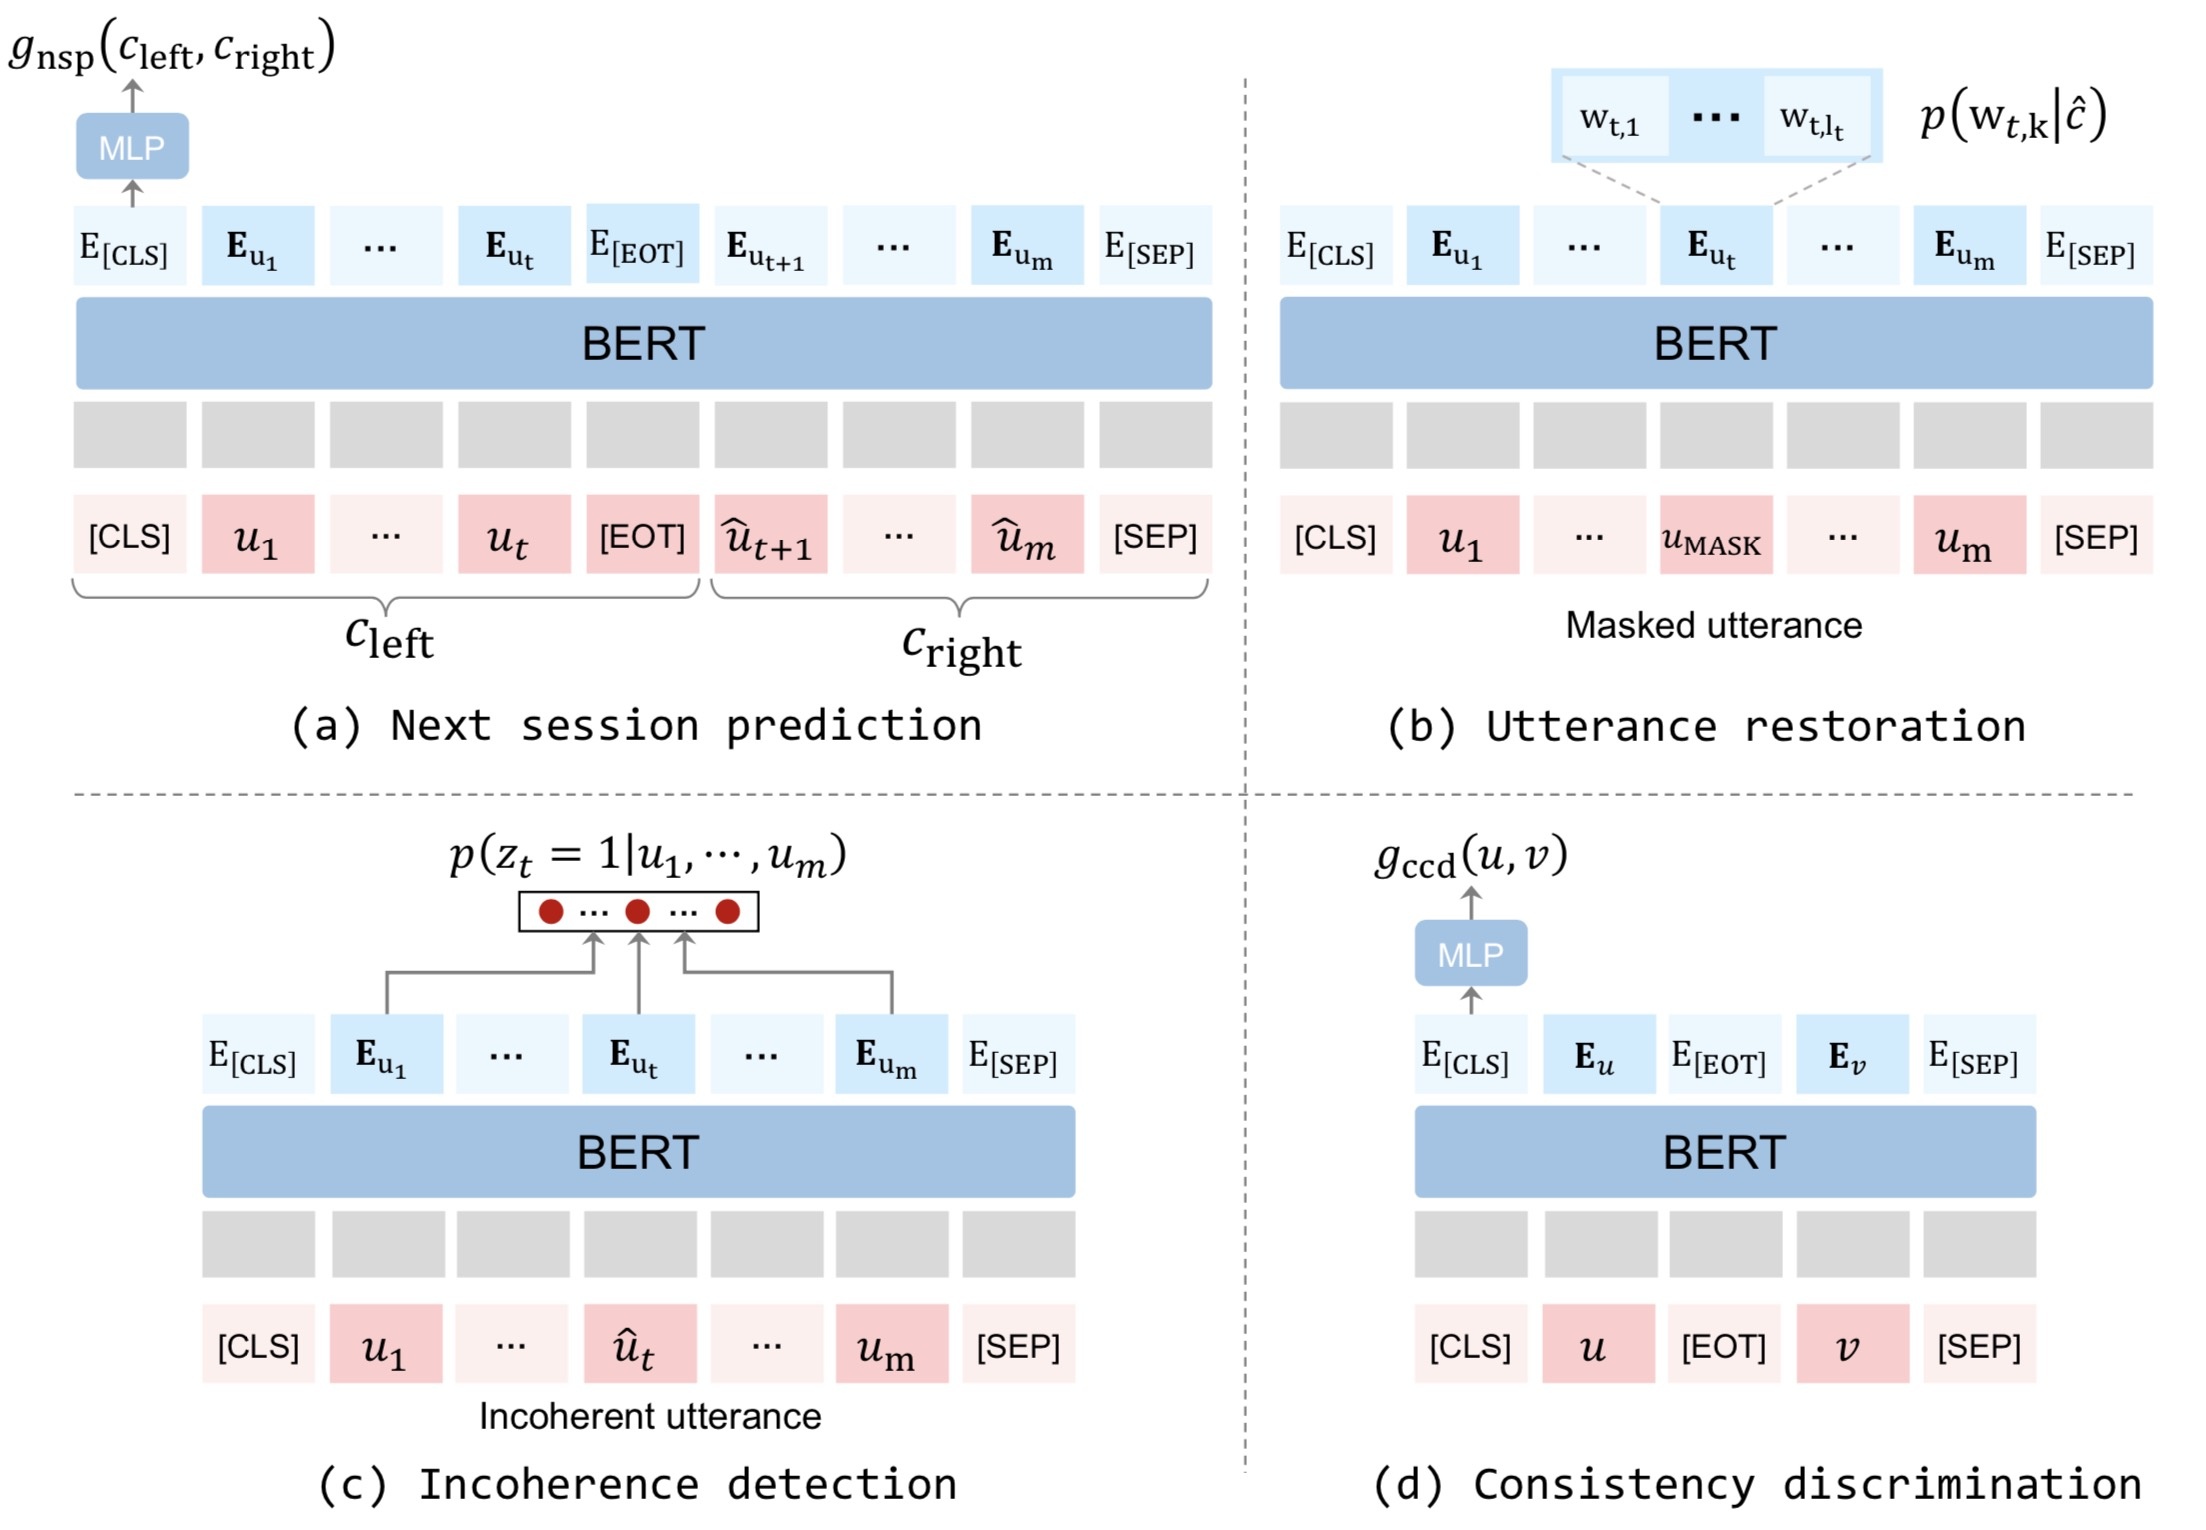
\includegraphics[width=0.9\linewidth]{Bert-SL.png}
        \end{center}
\end{frame}

\begin{frame}{Bert-SL}
Evaluation results on the two data sets.
\begin{center}
    \tiny
    \begin{tabular}{c|c|c|c|c|c|c|c}
\hline \multicolumn{1}{c|} { Metrics } & \multicolumn{4}{c|} { Ubuntu Corpus } & \multicolumn{3}{c} { E-commerce Corpus } \\
\cline { 2 - 8 } Models & $\mathrm{R}_{2} @ 1$ & $\mathrm{R}_{10} @ 1$ & $\mathrm{R}_{10} @ 2$ & $\mathrm{R}_{10} @ 5$ & $\mathrm{R}_{10} @ 1$ & $\mathrm{R}_{10} @ 2$ & $\mathrm{R}_{10} @ 5$ \\
\hline

\hline BERT (Whang et al., 2020) & 0.954 & 0.817 & 0.904 & 0.977 & 0.610 & 0.814 & 0.973 \\
SA-BERT (Gu et al., 2020) & 0.965 & 0.855 & 0.928 & 0.983 & 0.704 & 0.879 & 0.985 \\
BERT-VFT (Whang et al., 2020) & $-$ & 0.855 & 0.928 & 0.985 & $-$ & $-$ & $-$ \\
BERT-VFT (Ours) & 0.969 & 0.867 & 0.939 & 0.987 & 0.717 & 0.884 & 0.986 \\
\hline BERT-SL & $\mathbf{0 . 9 7 5}^{*}$ & $\mathbf{0 . 8 8 4}^{*}$ & $\mathbf{0 . 9 4 6}^{*}$ & $\mathbf{0 . 9 9 0}^{*}$ & $\mathbf{0 . 7 7 6}^{*}$ & $\mathbf{0 . 9 1 9}^{*}$ & 0.991 \\
\hline
\end{tabular}

\begin{tabular}{l|c|c|c|c|c|c|c}
\hline \multirow{} { Models } & \multicolumn{4}{|c|} { Ubuntu Corpus } & \multicolumn{3}{|c} { E-Commerce Corpus } \\
\cline { 2 - 8 } Metrics & $\mathrm{R}_{2} @ 1$ & $\mathrm{R}_{10} @ 1$ & $\mathrm{R}_{10} @ 2$ & $\mathrm{R}_{10} @ 5$ & $\mathrm{R}_{10} @ 1$ & $\mathrm{R}_{10} @ 2$ & $\mathrm{R}_{10} @ 5$ \\
\hline DualLSTM (Lowe et al., 2015) & 0.901 & 0.638 & 0.784 & 0.949 & 0.365 & 0.536 & 0.828 \\
DualLSTM-SL & $0.925^{*}$ & $0.724^{*}$ & $0.858^{*}$ & $0.969^{*}$ & $0.518^{*}$ & $0.722^{*}$ & $0.933^{*}$ \\
\hline ESIM (Chen \& Wang, 2019) & 0.950 & 0.796 & 0.874 & 0.975 & 0.570 & 0.767 & 0.948 \\
ESIM-SL & $0.963^{*}$ & $0.822^{*}$ & $0.909^{*}$ & $0.980^{*}$ & $0.623^{*}$ & $0.797^{*}$ & $0.969^{*}$ \\
\hline
\end{tabular}
\end{center}
\end{frame}


\begin{frame}{Embedding-based Retrieval in Facebook Search}
    \begin{center}
        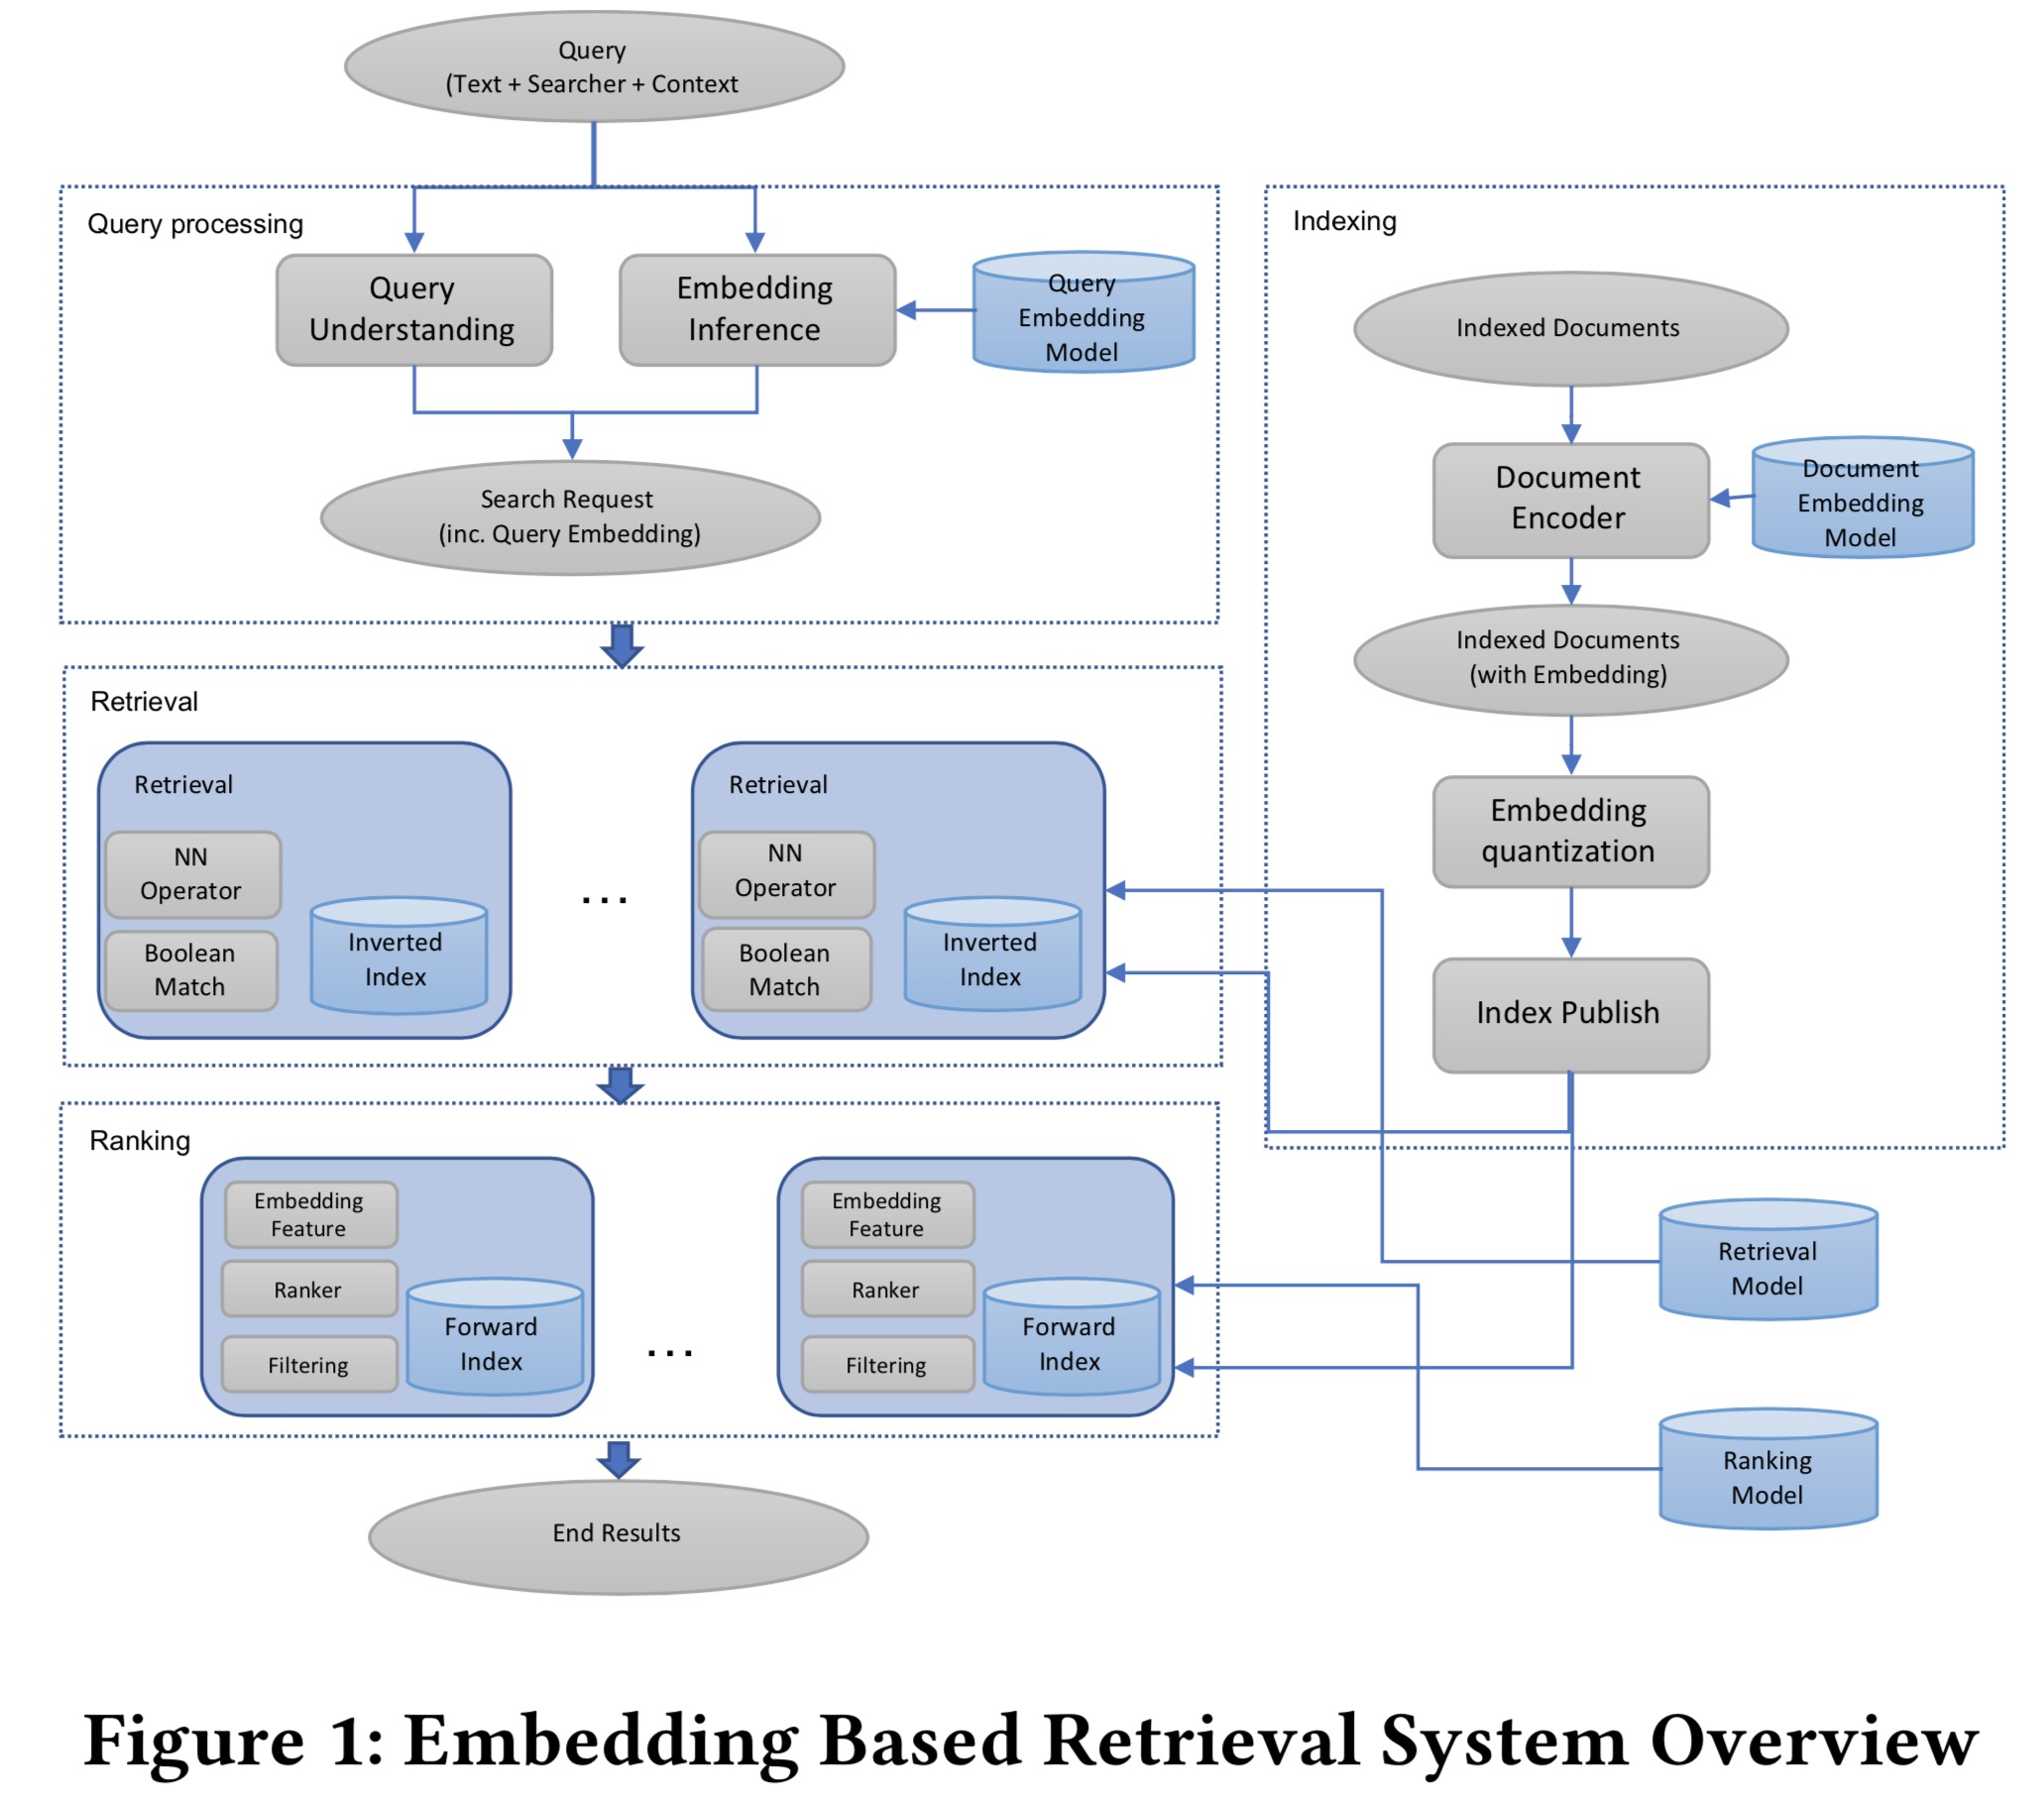
\includegraphics[width=0.7\linewidth]{Retrieval1.png}
    \end{center}
\end{frame}

\begin{frame}{Embedding-based Retrieval in Facebook Search}
    Wikipedia:
    
    Vector quantization works by dividing a large set of points (vectors) into groups having approximately the same number of points closest to them. Each group is represented by its centroid point, as in k-means and some other clustering algorithms.
    
    An approximate nearest neighbor search algorithm is allowed to return points, whose distance from the query is at most c times the distance from the query to its nearest points. The appeal of this approach is that, in many cases, an approximate nearest neighbor is almost as good as the exact one. 

\end{frame}

\begin{frame}{Embedding-based Retrieval in Facebook Search}
How to integrate embedding KNN and Boolean matching together:
 A query can be any Boolean expression on the terms. For example, the following query would return all the people that have john and smithe in the name, and live in Seattle or Menlo Park:
 
    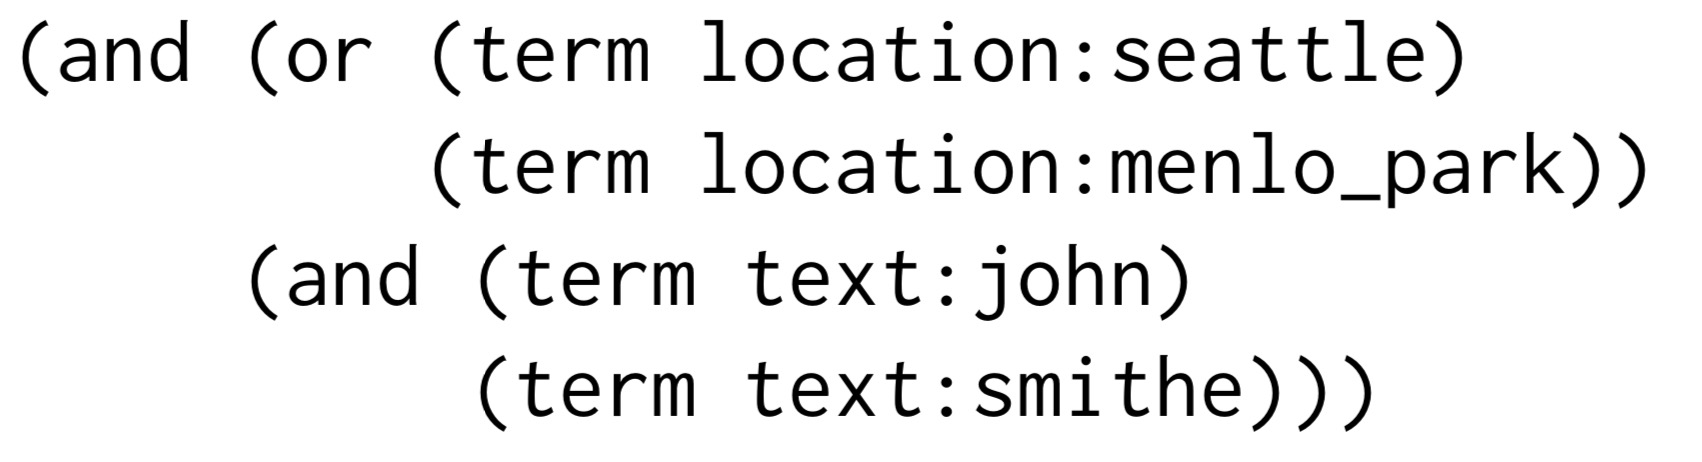
\includegraphics[width=0.7\linewidth]{Retrieval2.png}

To support $NN$, we extended the document representation to include embeddings, each with a given string key, and added a (nn <key> : radius <radius>) query operator which matches all documents whose $<$ key $>$ embedding is within the specified radius of the query embedding.

\end{frame}




\begin{frame}{TwinBERT}
\begin{center}
     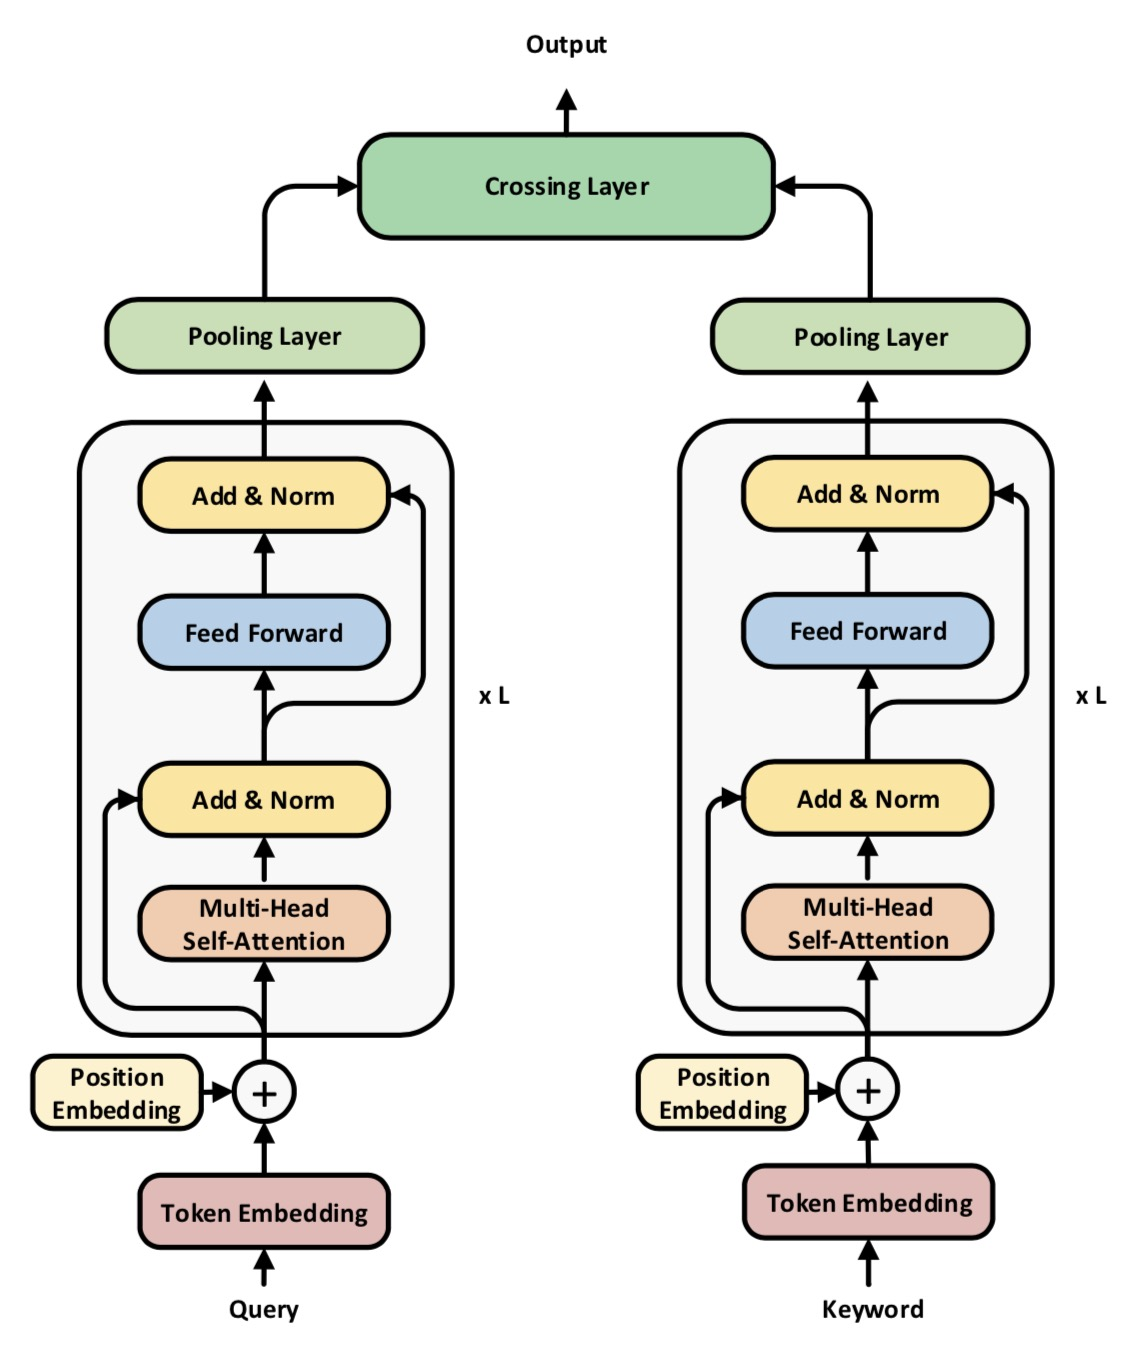
\includegraphics[width=0.55\linewidth]{TwinBert1.png}
\end{center}

\end{frame}


\begin{frame}{TwinBERT}
General Knowledge Distillation:
    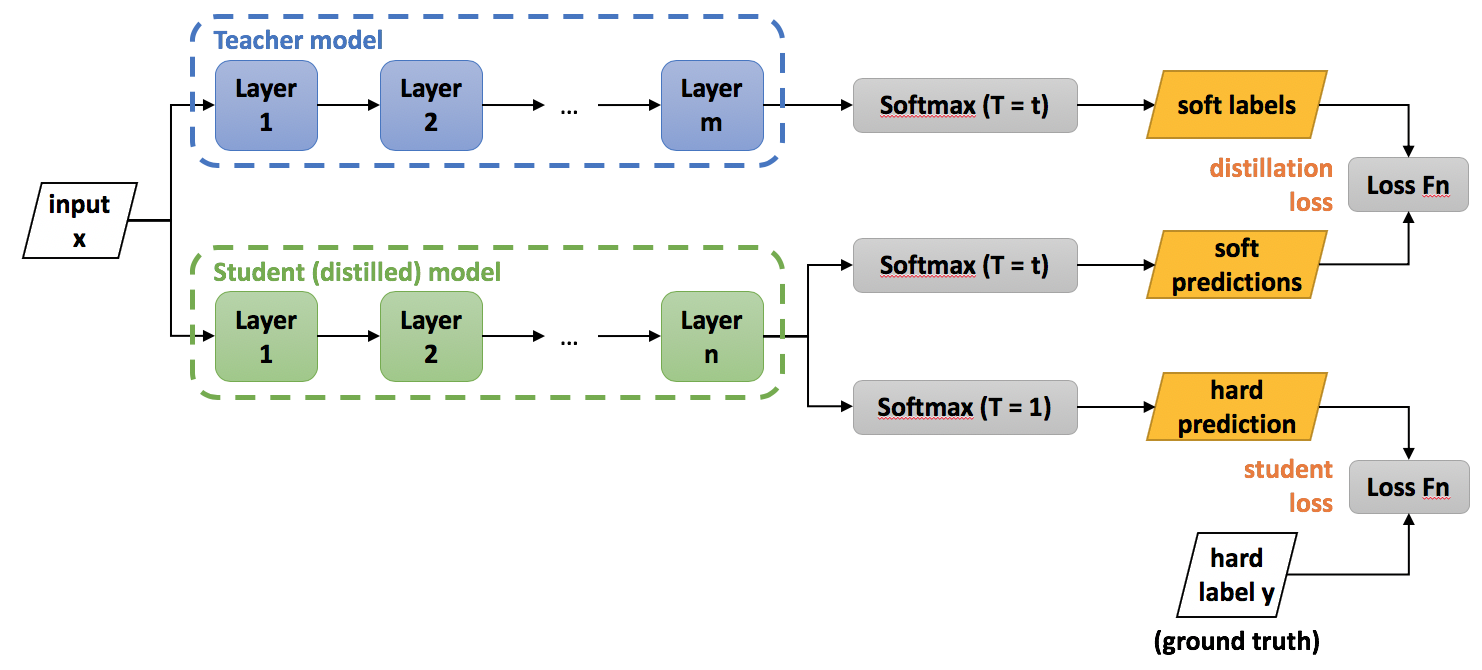
\includegraphics[width=1\linewidth]{knowledge_distillation.png}
\end{frame}

\begin{frame}{TwinBERT}
ROC-AUC of TwinBERT models comparing with CDSSM, BERT$_{3}$ and BERT$_{12}$ on two test sets
\begin{center}

\begin{tabular}{lll}
\hline Model & $\mathrm{AUC}_{1}$ & $\mathrm{AUC}_{2}$ \\
\hline C-DSSM & 0.8713 & 0.8571 \\
BERT $_{3}$ & 0.8995 & 0.9107 \\
TwinBERT $_{\text {cos }}$ & 0.8883 & 0.8743 \\
TwinBERT $_{\text {res }}$ & 0.9010 & 0.9113 \\
BERT $_{12}$ & 0.9011 & 0.9137 \\
\hline
\end{tabular}

\end{center}

\end{frame}



\begin{frame}{TwinBERT}
        Average inference time for TwinBERT, BERT $_{3}$ and BERT $_{12}$ over 1,000 queries. $Q$ EL refers to the number of query encoding loops.

    \begin{center}

\begin{tabular}{llll}
\hline Model & QEL & Memory & Inf. time (ms) \\
\hline TwinBERT $_{\cos }$ & 1 & $\sqrt{ }$ & 14 \\
TwinBERT $_{\text {res }}$ & 1 & $\sqrt{ }$ & 22 \\
TwinBERT res & 1 & & 1,077 \\
TwinBERT $_{\text {res }}$ & 100 & & 2,144 \\
BERT $_{3}$ & 100 & & 1,699 \\
BERT $_{12}$ & 100 & & 9,282 \\
\hline
\end{tabular}


 configuration: Intel® CoreTM i7- 4790 CPU @ 3.6GHz and 32.0GB memory
    \end{center}
\end{frame}

\end{document}


